\documentclass[11pt]{article}
\usepackage[T1]{fontenc}
\usepackage{lmodern,microtype}
\usepackage[a4paper,margin=28mm]{geometry}
\usepackage{amsmath,amssymb,amsthm,mathtools}
\usepackage{booktabs,array,enumitem}
\usepackage{tikz}
\usetikzlibrary{arrows.meta,positioning,calc,patterns}
\usepackage[numbers,sort&compress]{natbib}
\usepackage{xurl}
\usepackage[pdfencoding=auto,psdextra]{hyperref}
\hypersetup{colorlinks=true,linkcolor=blue!45!black,citecolor=blue!45!black,
urlcolor=blue!45!black,pdftitle={Existential-universal real sentences in the counting hierarchy},pdfauthor={OpenAI}}
\newtheorem{theorem}{Theorem}[section]
\newtheorem{proposition}[theorem]{Proposition}
\newtheorem{lemma}[theorem]{Lemma}
\newtheorem{corollary}[theorem]{Corollary}
\theoremstyle{definition}
\newtheorem{definition}[theorem]{Definition}
\newtheorem{example}[theorem]{Example}
\theoremstyle{remark}
\newtheorem{remark}[theorem]{Remark}
\numberwithin{equation}{section}
\newcommand{\R}{\mathbb R}
\newcommand{\C}{\mathbb C}
\newcommand{\Z}{\mathbb Z}
\newcommand{\Q}{\mathbb Q}
\newcommand{\N}{\mathbb N}
\newcommand{\F}{\mathbb F}
\newcommand{\ETR}{\mathsf{ETR}}
\newcommand{\EATR}{\exists\forall\mathbb R_{\mathrm{circ}}}
\newcommand{\existsR}{\exists\mathbb R}
\newcommand{\CH}{\mathsf{CH}}
\newcommand{\PP}{\mathsf{PP}}
\newcommand{\FP}{\mathsf{FP}}
\newcommand{\Pclass}{\mathsf P}
\newcommand{\PSPACE}{\mathsf{PSPACE}}
\newcommand{\NP}{\mathsf{NP}}
\newcommand{\Clevel}[1]{\mathsf C_{#1}\mathsf P}
\newcommand{\Flevel}[1]{\mathsf F_{#1}}
\DeclareMathOperator{\sgn}{sgn}
\DeclareMathOperator{\tr}{tr}
\DeclareMathOperator{\diag}{diag}
\DeclareMathOperator{\Res}{Res}
\DeclareMathOperator{\dist}{dist}
\DeclareMathOperator{\lcm}{lcm}
\newcommand{\norm}[1]{\left\lVert#1\right\rVert_1}
\newcommand{\abs}[1]{\left|#1\right|}
\newcommand{\ceil}[1]{\left\lceil#1\right\rceil}
\newcommand{\floor}[1]{\left\lfloor#1\right\rfloor}
\setlist[enumerate]{label=\textup{(\roman*)},leftmargin=2.1em}
\setlist[itemize]{leftmargin=1.6em}
\emergencystretch=1.5em

\title{Existential--universal real sentences\\in the counting hierarchy}
\author{OpenAI}
\date{October 4, 2026}
\begin{document}
\maketitle
\begin{abstract}
We prove that the existential theory of the reals lies in the counting
hierarchy. More generally, we show that the truth of existential--universal
sentences over the reals can be decided in a fixed level of the counting
hierarchy, even when the integer polynomials are given by arithmetic circuits.
\end{abstract}
\setcounter{tocdepth}{1}
\hypersetup{bookmarksdepth=2}
\begingroup\small\tableofcontents\endgroup
\clearpage
\section{Introduction}\label{sec:introduction}

A sentence with one existential and one universal real block asks whether
there is a real tuple for which every real tuple in a second block satisfies
specified polynomial conditions. We study the discrete language
$\EATR$ of true sentences
\begin{equation}\label{eq:input-sentence}
 \exists x\in\R^r\ \forall y\in\R^s:\ \Phi(x,y).
\end{equation}
Here $r,s\ge0$ are represented by explicit lists of variables, and $\Phi$
is an explicitly encoded Boolean formula using AND, OR, and NOT over atoms
$p=0$ and $p>0$. Each $p$ is given by an explicitly listed acyclic arithmetic
circuit with signed binary integer constants and gates $+,-,\times$.
Predecessor indices specify the gates; sharing is allowed, and there are
no division or exponentiation gates. All operations and comparisons in
\eqref{eq:input-sentence} are interpreted exactly. The input length $N$
is the total binary encoding length, and malformed encodings are rejected.

All computational bounds below are uniform bit-time bounds. Let $\PP$
denote polynomial-time probabilistic computation with fair random bits,
accepting exactly the yes-instances with probability greater than $1/2$.
The counting hierarchy, introduced by Wagner~\cite{Wagner1986}, is defined by
\[
 \Clevel0=\Pclass,\qquad
 \Clevel{j+1}=\bigcup_{A\in\Clevel j}\PP^A,
 \qquad \CH=\bigcup_{j\ge0}\Clevel j.
\]
Membership uses a fixed oracle language and a fixed uniform machine.

\begin{theorem}\label{thm:main}
There is an absolute integer $j$ such that
\[
                         \EATR\in\Clevel j.
\]
The level $j$ is independent of the input length, the numbers of variables,
the degrees of the circuit polynomials, and their coefficient magnitudes.
\end{theorem}

The existential theory of the reals, denoted $\ETR$, is the same decision
problem with only the existential block. Write $\existsR$ for the class
of languages polynomial-time many-one reducible to $\ETR$. Finer
accounting for this fragment gives $\ETR\in\Clevel{26}$ and hence
$\existsR\subseteq\Clevel{26}$; Theorem~\ref{thm:etr-bound} proves this
explicit bound. The main result allows a universal block of unrestricted
dimension as well.

\subsection{History and significance}

Tarski proved decidability of the first-order theory of real closed
fields~\cite{Tarski1951}. Collins's cylindrical algebraic decomposition
gave a geometric method for eliminating quantifiers~\cite{Collins1975},
and Canny established the polynomial-space upper bound for the existential
fragment~\cite{Canny1988}. For each fixed number of real quantifier blocks,
Renegar's decision bounds yield a polynomial-space algorithm
\cite[Theorem~1.1]{Renegar1992II}. This applies to the circuit encoding
above: the quartic reduction in Lemma~\ref{lem:quartic-fibers} preserves
the two quantifier blocks. Our theorem places this two-block language
in a fixed level of the counting hierarchy.
Real quantifier hierarchies distinguish the
number and order of blocks; Schaefer and \v{S}tefankovi\v{c} develop their
finite-encoding formulation~\cite{SchaeferStefankovic2025}.
The existential class already captures many geometric realization and
continuous feasibility problems; Schaefer, Cardinal, and Miltzow survey
these connections~\cite{SchaeferCardinalMiltzow2026}.

The counting hierarchy gives a way to decide some exact algebraic
questions without constructing their enormous intermediate integers.
Allender, B\"urgisser, Kjeldgaard-Pedersen, and Miltersen proved that
$\mathsf{PosSLP}$---positivity of the integer output of a division-free
straight-line program---belongs to $\CH$
\cite{AllenderBurgisserKjeldgaardPedersenMiltersen2009}.
Their modular-product and approximate Chinese-remainder techniques are
the counting tools behind our treatment of implicit polynomial families.
Every fixed counting level lies in $\PSPACE$: a depth-first simulation
enumerates random choices and answers the fixed-depth oracle queries
using polynomial space.

Recent counting-hierarchy bounds address other polynomial feasibility
problems. Andrews, Garg, and Schost place Hilbert's Nullstellensatz over
$\Q$ and several other fields in $\CH$~\cite{AndrewsGargSchost2026};
the common zeros there lie in an algebraic closure.
Balaji, Shirmohammadi, Tavenas, and Worrell prove counting-hierarchy
bounds for approximate polynomial satisfiability over $\Q$ and finite
fields~\cite{BalajiShirmohammadiTavenasWorrell2026}, where the question
is membership of zero in the Zariski closure of a polynomial image
over the algebraic closure.
Exact real quantification must also control the reality of solutions,
their attainment, and the dependence of a quantified fiber on its
parameters. These are the issues addressed by the argument here.

Our algebraic tools belong to the critical-point and deformation methods
of real algebraic geometry~\cite{BasuPollackRoy2006}. Multiplication
determinants are evaluated through the classical relation between
residues and traces~\cite{SchejaStorch1975,CattaniDickensteinSturmfels1996}.
We prove the needed identities and computational rules directly, including
their behavior under parameter specialization. These computational rules
apply to implicitly represented families that need not have short
coefficient lists or arithmetic circuits.

\subsection{From quantified fibers to short algebraic witnesses}

Fix the existential tuple $x$. Introducing gate and auxiliary variables
turns failure of $\Phi(x,y)$ into a real zero of a nonnegative quartic
$F(x,z)$, where $z$ includes $y$ and the auxiliaries. Thus we seek an
$x$ for which the fiber $F(x,\cdot)$ has no real zero. Call such an $x$
\emph{good}. Merely testing fibers does not provide a finite description
of a good parameter. The main geometric argument produces such descriptions.

For $u\ge0$, consider the minimum
\[
 m_x(u)=\min_{z\in\R^n}\left(\sum_{i=1}^n z_i^6+6uF(x,z)\right).
\]
The sixth powers keep bounded sublevel sets compact. It follows that
$m_x(u)$ remains bounded as $u\to\infty$ precisely when the fiber has
a zero. At a minimizing point the critical equations have pure fifth
powers as their leading terms. Their quotient algebra has dimension
$D=5^n$, and multiplication by the minimized polynomial has a monic
characteristic polynomial $Q(x,u,Y)$ satisfying
$Q(x,u,m_x(u))=0$.

This identity supplies a uniform growth test: $x$ is good precisely when
$m_x(v^{D+1})>v$ for all sufficiently large $v$. Form
\[
                         E(x,v)=Q(x,v^{D+1},v).
\]
The coefficient of $v^D$ is always $1$, so $E(x,\cdot)$ is never zero.
Partition parameter space into the sets on which $E(x,\cdot)$ has each
possible degree. On each such degree piece, polynomial root bounds give
a locally uniform threshold beyond which $E$ does not vanish.
Continuity of the minimum then makes goodness locally constant on that
piece. Introducing the reciprocal of its leading coefficient realizes
the piece as a closed algebraic set. Both the good and nongood parts
of this lift are closed.

A second minimization argument now extracts candidate coordinates.
Choose a compact sublevel set of a coercive polynomial with a good
point in its interior. Within this set, the good and nongood parts of
the lift are separated. Minimize the coercive polynomial plus a growing
nonnegative polynomial penalty that vanishes exactly on the lift,
restricting to a compact neighborhood that avoids the nongood part. A subsequence of
minimizers converges to a good point and is eventually interior to the
neighborhood, so these minimizers satisfy the unconstrained critical
equations. The highest parameter coefficients of their coordinate
characteristic polynomials therefore vanish at the limit coordinates.
This produces finitely indexed univariate polynomial families whose roots
contain the coordinates of a suitable witness, without computing the good part or its connected
components. Section~\ref{sec:two-blocks} proves this geometric
construction and completes the main theorem.

Two computational ingredients make these candidate coordinates usable.
First, all polynomials just described have degree and logarithmic
coefficient bounds with polynomial-length binary encodings, and their
finite-field evaluations lie at fixed counting levels. We call such
families \emph{controlled}. Sections~\ref{sec:counting} and
\ref{sec:algebra} establish their closure rules and the evaluation of
multiplication determinants without constructing the matrices.

Second, a chosen real root needs a short description even when its
polynomial has exponential degree. Derivative signs distinguish real
roots, as in Thom encodings~\cite{BasuPollackRoy2006}, but the full sign
string can be too long. Section~\ref{sec:labels} compresses that string
to a weighted integer sum with weights computed modulo a short prime,
and realizes the resulting
label by a polynomial positivity test. Every desired real root can
be isolated, including a root of a polynomial with multiplicities.
The sign approximation uses geometric products of the type studied
by Beigel, Reingold, and Spielman~\cite{BeigelReingoldSpielman1995}.
This arbitrary-root labeling rule and the coordinate construction
are reusable ingredients of the proof.

Finally, Section~\ref{sec:existential} proves an existential decision
procedure for controlled families. For a guessed coordinate description,
we use it twice: the described parameter set must be nonempty, and
it must contain no parameter with a zero of $F$. A suitable choice
of root labels singles out the good point constructed above. All
choices have polynomial total bit length, and all family constructions
have fixed depth. Counting over these choices therefore gives one
fixed level of the hierarchy.

\section{Counting and controlled polynomial families}\label{sec:counting}

The polynomials used below can have exponentially large degrees and
coefficients with exponentially many bits.  Their full expansions are
therefore unsuitable as algorithmic data.  We retain instead three
pieces of information: a degree bound, a coefficient-norm bound, and a
procedure for evaluation modulo a prime.  This section develops the
counting operations that preserve this description and recover the sign
of an integer from it.  The modular-product and approximate
Chinese-remainder methods follow the arithmetic approach of
Allender et al.~\cite[Section~4]{AllenderBurgisserKjeldgaardPedersenMiltersen2009};
we prove the forms, including the oracle bounds, that we need.

\subsection{Uniformity and counting}

Recall that $\Clevel{0}=\Pclass$ and
$\Clevel{a+1}=\bigcup_{A\in\Clevel{a}}\PP^A$.  Put
\[
 \Flevel{a}=\bigcup_{A\in\Clevel{a}}\FP^A.
\]
A function in $\Flevel{a}$ has polynomially bounded output length and is
computed in polynomial bit time with one fixed oracle in $\Clevel{a}$.
We call a function \emph{available} if it belongs to $\Flevel{a}$ for
some fixed $a$.  A decision made by such a function belongs to
$\Clevel{a+1}$: a probabilistic oracle machine can perform the same
computation and ignore its random bits.

The levels $\Clevel{a}$ are increasing and are closed under finite tagged
unions.  For the second assertion, induct on $a$, select the machine
indicated by the tag, and replace its oracle by the tagged union of the
finitely many lower-level oracles.  Padding with unused random bits
gives one polynomial random-bit bound.  Consequently, polynomial-time
computation using any fixed finite collection of available functions
again gives an available function.  This observation permits adaptive
calls; it makes no assertion that adaptive access to $\PP$ collapses to
$\PP$.

An integer or index is called \emph{short} if its binary encoding has
length bounded by a fixed polynomial in the relevant input length.
For a tuple, this means its total encoding length.  A short integer may
have exponentially large value.  Every index range below has a fixed
polynomial encoding bound, and every machine is fixed independently of
the input.  All algorithms are total: length and range checks prevent invalid
accesses, and undefined arithmetic operations receive fixed defaults.
Their asserted algebraic guarantees apply on the specified domains.

\begin{lemma}[Counting and summation]\label{lem:counting}
Fix $a\ge0$.  Let $b(w)$ and $s(w)$ be polynomially bounded nonnegative
integers computable in polynomial time.  If $A(w,i)$, for
$i\in\{0,1\}^{b(w)}$, is a predicate computable in $\Flevel{a}$, then
\[
 C(w)=\#\{i\in\{0,1\}^{b(w)}:A(w,i)\}
\]
is in $\Flevel{a+1}$.  Existential and universal quantification over
these indices are also in $\Flevel{a+1}$.

If $f(w,i)$ is in $\Flevel{a}$ and $0\le f(w,i)<2^{s(w)}$, then
$\sum_i f(w,i)$ is in $\Flevel{a+1}$.  The same conclusion holds for
sums modulo a positive short integer.
\end{lemma}

\begin{proof}
Write $b=b(w)$.  To test $C(w)>t$ for $0\le t\le2^b$, use one fair
choice bit and $b$ further random bits.  On the first choice accept
exactly when $A(w,i)$ holds; on the second accept on exactly $2^b-t$
of the $b$-bit strings.  There are
\[
 C(w)+2^b-t
\]
accepting choices, a strict majority precisely when $C(w)>t$.
The computation of $A$ is polynomial time with a fixed
$\Clevel{a}$ oracle, so the threshold language lies in
$\Clevel{a+1}$.  Binary search recovers $C(w)$, whose encoding uses at
most $b+1$ bits.  Unused random bits can pad this machine to a fixed
polynomial bound without changing its majority test.

The two quantified predicates follow by comparing the count with $0$
or $2^b$.  For summation, count pairs $(i,j)$ with
$j\in\{0,1\}^{s(w)}$ and $j<f(w,i)$.  The resulting integer has at most
$b+s(w)+1$ bits.  Reduction modulo a short modulus takes polynomial bit
time.  Restrictions on the indices may be included in the predicate or
implemented by zero summands.
\end{proof}

A sum over a tuple of indices uses one application of
Lemma~\ref{lem:counting}, as long as the tuple has polynomial total
length.  In particular, the number of counting levels does not grow
with the number of coordinates in a grid.

\begin{lemma}[Products in a finite field]\label{lem:field-product}\label{lem:product}
Fix $a\ge0$.  Let $p$ be a prime of polynomial bit length and let $b(w)$
be polynomially bounded and computable in polynomial time.  Suppose
$f(w,p,i)\in\F_p$, for $i\in\{0,1\}^{b(w)}$, is computable in
$\Flevel{a}$.  Then
\[
 \prod_{i\in\{0,1\}^{b(w)}} f(w,p,i)\pmod p
\]
is computable in $\Flevel{a+4}$.  A restricted index range can be used
by assigning factor $1$ outside it.  The algorithm can be made total,
with a fixed default when $p$ is not prime.
\end{lemma}

\begin{proof}
Primality can be tested in $\Flevel{1}$ by quantifying over possible
divisors.  For prime $p$, the multiplicative group $\F_p^*$ is cyclic.
Here is the elementary argument.  Let $L$ be the least common multiple
of the element orders.  For each prime power dividing $L$, a power of
some group element has exactly that prime-power order.  The product of
these elements has order $L$, since the orders are pairwise coprime.
Thus $L\le p-1$.  Every nonzero field element is a root of $z^L-1$, so
$p-1\le L$ by the polynomial root bound.  Hence $L=p-1$.

A nonzero $\gamma\in\F_p$ is a generator precisely when
\[
 \gamma^e\ne1\pmod p\qquad(1\le e\le p-2).
\]
Each power is computable in polynomial bit time.  By
Lemma~\ref{lem:counting}, the universal test is in $\Flevel{1}$.
An existential search over a short interval of candidates, followed by
binary search, therefore finds the least generator in $\Flevel{2}$.
For $p=2$ the displayed range is empty and $\gamma=1$.

First test whether any factor is zero, in which case the product is
zero.  Otherwise, each factor has a unique discrete logarithm
$e_i\in\{0,\ldots,p-2\}$ satisfying
\[
 \gamma^{e_i}=f(w,p,i)\pmod p.
\]
Existential searches over intervals, again followed by binary search,
recover $e_i$ in $\Flevel{\max(a,2)+1}$.  Summation puts
$\sum_i e_i$ in $\Flevel{\max(a,2)+2}$.  This sum is short, since it is
less than $2^{b(w)}p$.  Reduce it modulo $p-1$ and raise $\gamma$ to the
resulting exponent.  Since $\max(a,2)+2\le a+4$, all operations,
including the zero test and primality check, fit the asserted level.
\end{proof}

If a function receives $p$ as an additional input, its polynomial bounds
may use $|w|+\operatorname{bitlength}(p)$.  An application on a smaller
input, however, must supply $p$ with length polynomial in that smaller
input.  We will distinguish such evaluation inputs from the data that
describe the underlying polynomial family.

\subsection{Polynomial families accessible by evaluation}

Counting and finite-field products allow algebraic constructions without
writing their coefficients.  We now specify exactly what is retained about a
polynomial, and prove that coefficient extraction and differentiation
are compatible with this information.  For an integer polynomial $V$,
write $\norm{V}$ for the sum of the absolute values of all its
coefficients, in all its indeterminates.

\begin{definition}[Controlled polynomial family]\label{def:controlled}
A family $V_w\in\Z[X_1,\ldots,X_{n(w)}]$ is \emph{controlled} if the
following conditions hold.
\begin{enumerate}
\item The number $n(w)$ is polynomially bounded and computable in
polynomial time.
\item Nonnegative short integers $d(w),b(w),\lambda(w)$ are computable
in polynomial time and satisfy
\[
 \deg V_w\le d(w),\qquad \norm{V_w}\le2^{b(w)}.
\]
The zero polynomial is permitted and satisfies every nonnegative degree
bound.
\item For some fixed $a$, evaluation
\[
 (w,p,z)\longmapsto V_w(z)\bmod p,
 \qquad z\in\F_p^{n(w)},
\]
is in $\Flevel{a}$ on prime inputs $p>\lambda(w)$.  Field elements are
given by their least nonnegative binary representatives.
\end{enumerate}
The integers $d,b,\lambda$ depend only on $w$, not on the evaluation
prime or evaluation point.
\end{definition}

The word $w$ may include discrete choices and short indices.  When
members $V_{w,i}$ are summed or multiplied over an index set, the total
length of $i$ is bounded by a fixed polynomial in $|w|$, evaluation is
uniform in $i$, and we use bounds uniform over the allowed indices.
For example, if $|i|\le q(|w|)$ and each of $d,b,\lambda$ has at most
$r(|w|+|i|)$ bits, for fixed increasing polynomials $q,r$, then
$2^{r(|w|+q(|w|))}$ bounds all three uniformly.  This enlarged bound is
computable from $w$ alone, without enumerating the indices or testing
which members will be used.  All families in the argument arise from
fixed constructions; no machine describing a family is supplied as part
of the input.

\begin{lemma}[Finite-field coefficient extraction]\label{lem:field-coefficient}
Let $V_w(x,t)$ be a controlled family, where $x=(x_1,\ldots,x_h)$ is a
selected subset of its indeterminates and $t$ denotes the remaining
ones.  Let $\beta\in\N^h$ be a short index.  Then
$[x^\beta]V_w(x,t)$ is a controlled family, uniformly in $\beta$.
If the evaluation of $V$ is in $\Flevel{a}$, the coefficient evaluations
are in $\Flevel{a+1}$, with cutoff $\max(\lambda,d+1)$, degree bound
$d$, and coefficient-norm bound $2^b$.
\end{lemma}

\begin{proof}
Return the zero polynomial if some $\beta_i>d$ or $|\beta|>d$.
Otherwise let $p>\max(\lambda,d+1)$ be prime and specialize $t$ to a
point of the corresponding prime field.  In $\F_p$,
\begin{equation}\label{eq:field-coefficient}
 [x^\beta]V_w(x,t)
 =(p-1)^{-h}\sum_{z\in(\F_p^*)^h} V_w(z,t)z^{-\beta}.
\end{equation}
To see this, expand $V$ in monomials.  The sum of $z^e$ over
$\F_p^*$ is zero unless $p-1$ divides $e$, in which case it is $p-1$.
For each coordinate, the difference between a monomial exponent and
$\beta_i$ lies strictly between $-(p-1)$ and $p-1$; the only multiple
possible is zero.  This proves the identity.  The scalar $p-1$ is
nonzero in the field.

Since $h\le n(w)$ is polynomially bounded in $|w|$, the tuple $z$
uses $h\operatorname{bitlength}(p)$ bits, polynomial in the evaluation
input length.  This tuple is internal to one evaluation procedure; it
is not a family index used to define a new prime cutoff.  The cutoff
remains $\max(\lambda(w),d(w)+1)$, regardless of $p$.
The nonzero-coordinate restrictions can be enforced by zero summands,
and powers and inverses are computable in polynomial bit time.
Lemma~\ref{lem:counting} therefore evaluates the sum in
$\Flevel{a+1}$.  Extracting coefficients only removes terms and their
$x$ exponents, so it does not increase degree or coefficient norm.  If
$h=0$, the identity is the single empty-tuple summand and the same
conclusion holds.
\end{proof}

\begin{proposition}[Closure of controlled families]\label{prop:controlled-closure}
Controlled families are preserved by each of the following operations,
applied a fixed number of times:
\begin{enumerate}
\item sums and products over short index sets, with uniform bounds on
the summands or factors;
\item powers with short nonnegative exponents computable in polynomial
time, and substitution of controlled polynomials for indeterminates;
\item extraction of indexed coefficients in any subset of the
indeterminates, and differentiation in one variable to a short indexed
nonnegative order.
\end{enumerate}
In the first operation the index domain is specified in polynomial time;
more generally, an available predicate $A(w,i)$ may restrict the indices
when polynomial-time uniform bounds for the unrestricted domain are
retained.  This predicate depends only on the primary word and the
family index, not on an evaluation prime or evaluation point.  All resulting
bounds and prime cutoffs are computable in polynomial bit time from the
primary family data.  In particular, they are independent of evaluation
primes.
\end{proposition}

\begin{proof}
For sums and products, suppose there are at most $L$ members, with
common degree bound $d$, norm bound $2^b$, and cutoff $\lambda$, where
$L$ is short and computable in polynomial time.  The triangle inequality
and submultiplicativity of coefficient norm give the bounds
\[
 \begin{array}{c|cc}
 &\text{degree}&\text{logarithmic norm bound}\\ \hline
 \text{sum}&d&b+\operatorname{bitlength}(L+1)\\
 \text{product}&Ld&Lb.
 \end{array}
\]
Empty sums and products are $0$ and $1$.  The bounds can be enlarged in
these cases if necessary.  Evaluations follow from
Lemmas~\ref{lem:counting} and~\ref{lem:field-product}.  An available
restriction is tested while evaluating a summand or factor, with the
neutral value used outside the range.  Tagged unions combine the fixed
collection of evaluation and restriction oracles.

For a nonnegative short exponent $e$, the bounds for $V^e$ are $ed$ and
$eb$; when $e=0$, the polynomial is $1$.  Evaluation uses ordinary
modular powering with a short exponent.  Suppose next that $V$ has
bounds $d,2^b$, and that each substitute has bounds $d',2^{b'}$.
Termwise substitution gives degree at most $dd'$ and norm at most
\[
 2^b(2^{b'})^d=2^{b+db'}.
\]
Include unchanged variables among the substitutes when needed.
Evaluation first computes the polynomially many substituted values and
then evaluates $V$ at them.  The maximum of the cutoffs of these calls
is a suitable cutoff for the composition.  Uniform bounds over a
polynomially indexed collection of substitutes are taken before choosing
the evaluation prime, as in Definition~\ref{def:controlled}.

Coefficient extraction is Lemma~\ref{lem:field-coefficient}.  For
differentiation, write $x$ for the selected variable and $t$ for the
others.  If the requested order $j$ exceeds $d$, return zero.  For
$0\le j\le d$ we have
\begin{equation}\label{eq:indexed-derivative}
 \frac{\partial^j V}{\partial x^j}(x,t)
 =\sum_{k=j}^d (k)_j\,[x^k]V(x,t)\,x^{k-j},
 \qquad (k)_j=\prod_{v=0}^{j-1}(k-v).
\end{equation}
The empty product for $j=0$ is $1$.  Modulo a prime above
$\max(\lambda,d+1)$, the coefficient polynomials are available by
Lemma~\ref{lem:field-coefficient}; the falling factorials are available
by Lemma~\ref{lem:field-product}; and the outer sum is available by
Lemma~\ref{lem:counting}.  All indices are short, even when $j$ or $d$
is exponentially large.  For example, an $\Flevel{a}$ evaluator for $V$
gives an $\Flevel{a+5}$ evaluator for the derivative by these bounds.
Differentiation does not increase degree, and
\[
 \left\|\frac{\partial^j V}{\partial x^j}\right\|_1
 \le\max(d,1)^d\norm{V}
 \le 2^{b+d^2+1}.
\]
Thus the derivative has short, polynomial-time computable bounds.

Every arithmetic operation used to obtain these degree, norm, and
cutoff bounds is on short integers.  A fixed number of the constructions
therefore leaves all bounds short and all evaluation procedures at a
fixed counting level.  The hypothesis of fixed nesting is essential:
the proposition does not assert closure under an input-dependent
sequence of successive counting operations.
\end{proof}

Ordinarily encoded short integers are controlled constant families.
The same holds for much larger constants such as $2^e$ with a short
nonnegative exponent $e$: its logarithmic norm bound is $e$, and its
residue is obtained by modular powering.  Such a constant is used
through its residues and bounds, not through its full binary expansion.

\subsection{Recovering an integer sign}

The closure rules give modular evaluations and magnitude bounds for
integer families, including integers too large to write down.  It
remains to recover their signs.  A collection of prime residues
mathematically determines such an integer, but constructing its full
Chinese-remainder representative may require exponentially many bits.
We instead approximate the integer divided by a sufficiently large
prime product, modulo one.  Successive doublings bring a nonzero
quotient far enough from zero to reveal its sign.

\begin{proposition}[Sign from residues]\label{prop:crt-sign}
Let $X(w)\in\Z$ and suppose that nonnegative short integers $m(w)$ and
$\lambda(w)$ are computable in polynomial time, with
$|X(w)|\le2^{m(w)}$.  Define
\begin{equation}\label{eq:crt-bounds}
 Z=\max(16,m,\lambda),\qquad Y=2Z^4.
\end{equation}
If $X(w)\bmod p$, represented in $\{0,\ldots,p-1\}$, is uniformly
computable in $\Flevel{a}$ for primes $\lambda<p\le Y$, then
$\sgn X(w)$ is in $\Flevel{\max(a,5)+3}$.
\end{proposition}

\begin{proof}
Let $\mathcal P$ consist of the primes $\lambda<p\le Y$, and write
$\Pi=\prod_{p\in\mathcal P}p$.  The product $\Pi$ is used only in the
proof, not stored by the algorithm.  We first show that it is large
enough.  Since $Y$ is even,
\[
 \binom{Y}{Y/2}\ge\frac{2^Y}{Y+1}.
\]
The exponent of a prime $p$ in this binomial coefficient is the sum of
\[
 \left\lfloor\frac{Y}{p^j}\right\rfloor
 -2\left\lfloor\frac{Y/2}{p^j}\right\rfloor\in\{0,1\}
 \qquad(p^j\le Y).
\]
Consequently, the total power of any one prime dividing the binomial
coefficient is at most $Y$.  If $\pi(Y)$ is the number of primes at most
$Y$, then
\[
 \pi(Y)\log_2Y\ge Y-\log_2(Y+1)\ge Y/2.
\]
Because $\log_2Y\le5Z$, at least $Z^3/5$ primes are at most $Y$.
Removing the at most $\lambda\le Z$ primes below the cutoff leaves at
least $3Z$ primes.  With $b_Y=\operatorname{bitlength}(Y)$, we obtain
\begin{equation}\label{eq:crt-product-bounds}
 2^{3Z}\le\Pi\le2^{Yb_Y},\qquad |X/\Pi|<1/6.
\end{equation}

For each $0\le k\le Yb_Y+1$ and $p\in\mathcal P$, set
\begin{equation}\label{eq:crt-residues}
 c_{p,k}=2^kX(\Pi/p)^{-1}\pmod p,
 \qquad 0\le c_{p,k}<p.
\end{equation}
To compute $(\Pi/p)\bmod p$, take a product modulo $p$ over all other
primes in $\mathcal P$.  The primality and range tests are in
$\Flevel{1}$, so Lemma~\ref{lem:field-product} puts this product in
$\Flevel{5}$.  It is nonzero.  Modular inversion, modular powering,
and the assumed residues of $X$ therefore compute $c_{p,k}$ in
$\Flevel{\max(a,5)}$.  All arguments are short, including $k$.

Chinese remaindering gives the identity
\begin{equation}\label{eq:crt-circle-identity}
 \sum_{p\in\mathcal P}\frac{c_{p,k}}p
 \equiv\frac{2^kX}{\Pi}\pmod1.
\end{equation}
Indeed, multiplying the difference by $\Pi$ gives an integer divisible
by every prime in $\mathcal P$.  Put $B_Y=b_Y+10$ and form the short
dyadic number
\[
 w_k=2^{-B_Y}\left(
 \sum_{p\in\mathcal P}
 \left\lfloor\frac{2^{B_Y}c_{p,k}}p\right\rfloor
 \bmod 2^{B_Y}\right)\in[0,1).
\]
There are fewer than $2^{b_Y}$ summands, each rounded down by less than
$2^{-B_Y}$.  Thus, for circular distance
$\operatorname{dist}_{\R/\Z}(u,v)=\min_{\ell\in\Z}|u-v-\ell|$,
\begin{equation}\label{eq:crt-circle-error}
 \operatorname{dist}_{\R/\Z}
 \left(w_k,\frac{2^kX}{\Pi}\right)<2^{-10}.
\end{equation}
The scaled sum has at most $2b_Y+11$ bits, and
Lemma~\ref{lem:counting} computes $w_k$ in
$\Flevel{\max(a,5)+1}$.

Call $k$ \emph{flagged} when $1/8\le w_k\le7/8$.  If $X=0$, every
$c_{p,k}$ is zero, so no index is flagged.  If $X\ne0$, let $k_0$ be
the first index with $|2^{k_0}X/\Pi|\ge1/6$.
Equation~\eqref{eq:crt-product-bounds} implies that
$0<k_0\le Yb_Y+1$, and minimality gives
\[
 1/6\le|2^{k_0}X/\Pi|<1/3.
\]
The error bound therefore makes $k_0$ flagged.

At the first flagged index $k$, we have $k\le k_0$ and
$|2^kX/\Pi|<1/3$.  If $X>0$, its residue modulo one lies in $(0,1/3)$;
if $X<0$, the residue lies in $(2/3,1)$.  An approximation that wraps
across $0=1$ must be within $2^{-10}$ of that endpoint and so cannot be
flagged.  It follows that $w_k<1/2$ in the positive case and $w_k>1/2$
in the negative case.  Figure~\ref{fig:crt-sign} records this separation.

\begin{figure}[tb]
\centering
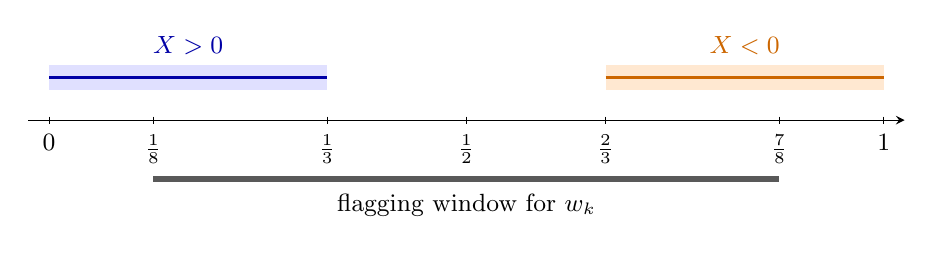
\begin{tikzpicture}[x=10.6cm,y=1cm,>=stealth,font=\small]
 \fill[blue!12] (0,.38) rectangle (0.333333,.7);
 \fill[orange!18] (0.666667,.38) rectangle (1,.7);
 \draw[blue!65!black,thick] (0,.54)--(0.333333,.54);
 \draw[orange!80!black,thick] (0.666667,.54)--(1,.54);
 \node[blue!65!black,above] at (.166667,.7) {$X>0$};
 \node[orange!80!black,above] at (.833333,.7) {$X<0$};
 \draw[->] (-.025,0)--(1.025,0);
 \foreach \x/\lab in {0/0,0.125/{\frac18},0.333333/{\frac13},0.5/{\frac12},0.666667/{\frac23},0.875/{\frac78},1/1}
  {\draw (\x,.045)--(\x,-.045);\node[below] at (\x,-.06) {$\lab$};}
 \draw[black!65,line width=2pt] (.125,-.75)--(.875,-.75);
 \node[below] at (.5,-.82) {flagging window for $w_k$};
\end{tikzpicture}
\caption{At the first flagged index, the true residue
$(2^kX/\Pi)\bmod1$ lies in the left interval for $X>0$ and the right
interval for $X<0$.  The circular error of $w_k$ is less than $2^{-10}$.
The flagging window excludes any approximation that wraps across $0=1$,
so the side of $1/2$ determines the sign.}
\label{fig:crt-sign}
\end{figure}

The first-flag condition uses one universal quantifier over smaller
short indices, raising the level for $w_k$ by one.  Existentially
quantifying a first flagged index with $w_k<1/2$, or with $w_k>1/2$,
raises it once more.  These tests return the positive or negative sign;
if neither succeeds, return zero.  This is the asserted
$\Flevel{\max(a,5)+3}$ procedure.
\end{proof}

\begin{corollary}[Signs of controlled integers]\label{cor:controlled-sign}
If a controlled family has no indeterminates, its sign is available,
uniformly in any short indices belonging to its input word.
\end{corollary}

\begin{proof}
Apply Proposition~\ref{prop:crt-sign} with the logarithmic norm bound
$b$ in place of $m$ and with the family's cutoff $\lambda$.
\end{proof}

We can now manipulate polynomials through short bounds and modular
evaluation procedures.  The next step is to show that a characteristic
polynomial of multiplication in a finite polynomial quotient admits
exactly this description, even when the quotient has exponentially
large rank.

\section{Multiplication determinants without large matrices}
\label{sec:algebra}

The geometric constructions below produce polynomial systems whose
leading terms are pure powers.  Their quotient algebras have explicit
monomial bases, but those bases can be exponentially large.  The goal
of this section is to compute characteristic polynomials of
multiplication in these algebras as controlled families, without
constructing the multiplication matrices.  We first express a trace
as a coefficient, and then recover characteristic coefficients from
traces by fixed-depth finite-field computations.

\subsection{A basis and a coefficient functional}

Let $S$ be a commutative ring with identity, let $n\ge1$ and $\ell\ge2$,
and suppose that $r_1,\ldots,r_n\in S[x_1,\ldots,x_n]$ satisfy
$\deg_x r_i<\ell$.  Set
\begin{equation}\label{eq:quotient-algebra}
 f_i=x_i^\ell-r_i,\qquad
 \mathcal A=S[x_1,\ldots,x_n]/(f_1,\ldots,f_n),\qquad
 D=\ell^n,\qquad \tau=(\ell-1,\ldots,\ell-1).
\end{equation}
For a multi-index $a$, write $|a|=\sum_i a_i$ and
$x^a=\prod_i x_i^{a_i}$.  We will show that the $D$ monomials
$x^a$ with $0\le a_i<\ell$ form an $S$-basis of $\mathcal A$.

We use formal Laurent sums whose total degrees are bounded above and
whose support in each total degree is finite.  Addition and
multiplication are well defined: for any prescribed total degree,
only finitely many pairs of degrees and finitely many terms can
contribute.  Since $r_i x_i^{-\ell}$ has total degree at most $-1$,
its geometric series is such a Laurent sum.  Define the $S$-linear
functional
\begin{equation}\label{eq:laurent-functional}
 \mathcal L(v)=
 [x_1^{-1}\cdots x_n^{-1}]
 v(x)\prod_{i=1}^n
 \left(x_i^{-\ell}\sum_{j\ge0}
       (r_i(x)x_i^{-\ell})^j\right).
\end{equation}
This is a formal coefficient extraction, requiring neither convergence
nor division in $S$.  It is a concrete residue formula of the type
studied in \cite{CattaniDickensteinSturmfels1996}; we prove the facts
needed here directly over $S$.

\begin{lemma}\label{lem:monomial-basis}
The functional $\mathcal L$ vanishes on $(f_1,\ldots,f_n)$ and hence
descends to $\mathcal A$.  If $\deg_x v\le n(\ell-1)$, then
\begin{equation}\label{eq:low-degree-functional}
 \mathcal L(v)=[x^\tau]v.
\end{equation}
The algebra $\mathcal A$ is a free $S$-module with basis
$\{x^a:0\le a_i<\ell\}$.
\end{lemma}

\begin{proof}
Multiplying the expression in Equation~\eqref{eq:laurent-functional}
by $f_i=x_i^\ell-r_i$ cancels its $i$th geometric factor.  In the
remaining expression, every exponent of $x_i$ is nonnegative:
the other denominators are powers of the other variables, while all
numerators are polynomials.  Its coefficient with $x_i$-exponent $-1$
is zero.  Thus $\mathcal L(vf_i)=0$ for every polynomial $v$.

Expanding all the geometric factors gives the finite sum
\begin{equation}\label{eq:laurent-coefficient-sum}
 \mathcal L(v)=\sum_{j\in\mathbb Z_{\ge0}^n}
 [x^{\tau+\ell j}]\left(v\prod_{i=1}^n r_i^{j_i}\right).
\end{equation}
The target degree in a summand is $n(\ell-1)+\ell|j|$, whereas the
numerator has degree at most $\deg_x v+(\ell-1)|j|$.  A nonzero
summand therefore requires
\begin{equation}\label{eq:residue-truncation}
 |j|\le\deg_x v-n(\ell-1).
\end{equation}
This proves finiteness and Equation~\eqref{eq:low-degree-functional}.

The relations $x_i^\ell=r_i$ express every monomial as a linear
combination of the proposed basis elements: each replacement strictly
decreases total $x$-degree.  For independence, consider
\[
 P_{a,b}=\mathcal L(x^a x^{\tau-b}),
 \qquad a,b\in\{0,\ldots,\ell-1\}^n.
\]
Equation~\eqref{eq:low-degree-functional} gives $P_{a,b}=0$ if
$|a|<|b|$, and $P_{a,b}=\delta_{a,b}$ if $|a|=|b|$.
Ordering both index sets by total degree makes $P$ block triangular
with identity diagonal blocks.  It is therefore invertible over $S$.
Pairing any linear relation among the proposed basis elements against
all $x^{\tau-b}$ forces all its coefficients to be zero.
\end{proof}

\subsection{A trace formula and its spectral consequences}

Let $M_v$ denote the matrix of multiplication by the class of
$v\in S[x]$ in this basis, and put
\begin{equation}\label{eq:jacobian}
 J(x)=\det\bigl(\partial_j f_i(x)\bigr)_{1\le i,j\le n}.
\end{equation}
The following classical trace--residue identity is associated with
Scheja and Storch \cite{SchejaStorch1975}; see also
\cite[Author version, Equation~(4.7)]{CattaniDickensteinSturmfels1996}.
Its proof uses the dual-basis
property of a Bezoutian, a construction developed further in
\cite[Section~3.3]{ElkadiMourrain2005}.  The explicit proof matters here because
we need arbitrary coefficient rings and specialization at multiple
zeros.

\begin{proposition}[Trace formula]\label{prop:trace}
For the algebra in Equation~\eqref{eq:quotient-algebra}, over every
commutative ring $S$ with identity,
\begin{equation}\label{eq:trace-formula}
 \operatorname{tr}(M_v)=\mathcal L(vJ)
 \qquad(v\in S[x]).
\end{equation}
\end{proposition}

\begin{proof}
Introduce another set of variables $x'=(x'_1,\ldots,x'_n)$.
Changing one variable at a time gives polynomial divided differences
$W_{ij}(x,x')$ such that
\[
 f_i(x)-f_i(x')=\sum_{j=1}^n
 W_{ij}(x,x')(x_j-x'_j).
\]
Each $W_{ij}$ has combined $(x,x')$-degree at most $\ell-1$.
Let $W=\det(W_{ij})$.  In $\mathcal A\otimes_S\mathcal A$, the
left sides vanish, so multiplication by the adjugate matrix gives
\begin{equation}\label{eq:diagonal-annihilation}
 W(x,x')(x_j-x'_j)=0\qquad(1\le j\le n).
\end{equation}

Apply $\mathcal L$ in the second factor, writing this map as
$\mathcal L_{x'}$.  Since $\deg_{x'}W\le n(\ell-1)$,
Lemma~\ref{lem:monomial-basis} gives
$\mathcal L_{x'}(W)=[(x')^\tau]W$.  This coefficient is $1$.
Indeed, the part of combined degree $\ell-1$ in the divided-difference
matrix is diagonal, with $i$th diagonal entry
\[
 x_i^{\ell-1}+x_i^{\ell-2}x'_i+\cdots+(x'_i)^{\ell-1}.
\]
The contributions from the $r_i$ have combined degree at most
$\ell-2$.  To obtain the $(x')^\tau$ coefficient, whose total
degree is $n(\ell-1)$, one must use the last term of every displayed
diagonal entry.  The target exhausts the combined-degree bound, so
no positive $x$-degree can occur in this coefficient.

Equation~\eqref{eq:diagonal-annihilation} now yields the reproducing
identity
\begin{equation}\label{eq:reproducing-identity}
 \mathcal L_{x'}\bigl(W(x,x')v(x')\bigr)=v(x)
 \quad\text{in }\mathcal A:
\end{equation}
within a product with $W$, each $x'_j$ can be replaced by $x_j$.
Expand $W=\sum_a x^a w_a(x')$ in the first monomial basis of the
tensor product.  Equation~\eqref{eq:reproducing-identity} says that
the $x^a$-coordinate of $v$ is $\mathcal L(w_a v)$.  In particular,
the $a$th diagonal entry of $M_v$ is $\mathcal L(w_a v x^a)$.
The multiplication map $\mathcal A\otimes_S\mathcal A\to\mathcal A$
identifies $\sum_a x^a w_a(x)$ with $W(x,x)$, so
\[
 \operatorname{tr}(M_v)
 =\mathcal L\!\left(v\sum_a x^a w_a(x)\right)
 =\mathcal L\bigl(vW(x,x)\bigr).
\]
On the diagonal $x'=x$, divided differences become derivatives;
hence $W(x,x)=J(x)$, proving the formula.
\end{proof}

Both the basis and the trace formula commute with every change of
coefficient ring.  In particular, parameters may be specialized and
coefficients reduced modulo a prime without assuming that the common
zeros are distinct.  The following elementary fact explains how the
characteristic polynomials will encode real critical values.

\begin{lemma}\label{lem:real-eigenline}
Suppose that the coefficients of the relations in
Equation~\eqref{eq:quotient-algebra} and of $v$ lie in $\mathbb C$,
and write $Q(y)=\det(yI-M_v)$.  Every common zero
$\xi\in\mathbb C^n$ of the $f_i$ satisfies $Q(v(\xi))=0$.
If all coefficients are real and $\eta$ is a simple real root of $Q$,
there is a common zero $\xi\in\mathbb R^n$ with $v(\xi)=\eta$.
Moreover, for any polynomial $g$ over $\mathbb C$,
\begin{equation}\label{eq:composition-determinant}
 M_{g(v)}=g(M_v),\qquad
 \det M_{g(v)}=\prod_{Q(\alpha)=0}g(\alpha),
\end{equation}
where the roots in the product are counted with multiplicity.
\end{lemma}

\begin{proof}
Evaluation at a common zero $\xi$ is a nonzero linear functional on
$\mathcal A$, since it sends $1$ to $1$.  It satisfies
$\operatorname{ev}_\xi(vw)=v(\xi)\operatorname{ev}_\xi(w)$,
so it is a left eigenvector of $M_v$ with eigenvalue $v(\xi)$.

For real coefficients, a simple real eigenvalue $\eta$ of the real
matrix $M_v$ has a one-dimensional real eigenspace.  Each coordinate
multiplication matrix $M_{x_i}$ commutes with $M_v$ and therefore
preserves this line.  Let $\xi_i\in\mathbb R$ be its scalar action
there.  Restricting the matrix identities
\[
 f_i(M_{x_1},\ldots,M_{x_n})=0,\qquad
 v(M_{x_1},\ldots,M_{x_n})=M_v
\]
to the line gives $f_i(\xi)=0$ and $v(\xi)=\eta$.
Finally, multiplication respects sums and products, giving the first
identity in Equation~\eqref{eq:composition-determinant}; triangularizing
$M_v$ over $\mathbb C$ gives the second.
\end{proof}

\subsection{Characteristic coefficients from finite-field evaluations}

We now turn the trace formula into a uniform computation.  All the
large sums below are indexed by tuples of polynomial bit length.
Each entire tuple is a single counting index; the number of its
coordinates does not increase the number of counting levels.
We state the evaluation bound separately, so that later applications
with elementary evaluators can retain their sharper level count.

\begin{proposition}[Indexed characteristic coefficients]
\label{prop:char-coeff}
Consider fixed families $r_1,\ldots,r_n,v\in\mathbb Z[x]$, indexed
by a word of length $N$.  Suppose that $n\ge1$ is polynomially bounded
and polynomial-time computable, that $\ell\ge2$ and $\Omega\ge0$
are short polynomial-time computable integers, and that
$\deg_x r_i<\ell$ and $\deg_x v\le\Omega$.  Put
\[
 f_i=x_i^\ell-r_i,\qquad
 J=\det(\partial_jf_i),\qquad
 D=\ell^n,\qquad L_0=D\Omega+n(\ell-1).
\]
For $a\ge0$, suppose that $v$, the indexed $r_i$, and $J$ can be
evaluated uniformly in $\Flevel{a}$ over prime fields with
\begin{equation}\label{eq:char-prime-bound}
 p>n(\ell-1)+\ell L_0+D^2+10.
\end{equation}
Additional short, polynomial-time computable lower cutoffs on $p$
are allowed.  Then, for every $0\le d\le D$,
\[
 [y^d]\det(yI-M_v)\pmod p
\]
is uniformly computable in $\Flevel{a+8}$ in this prime range.
All running-time and query-length bounds are polynomial in the
length of the input, including $p$ and the coefficient index $d$.
\end{proposition}

\begin{proof}
First compute the trace residues $t_k=\operatorname{tr}(M_v^k)\bmod p$
for short indices $1\le k\le D$.  By Proposition~\ref{prop:trace},
$M_v^k=M_{v^k}$, and Equation~\eqref{eq:laurent-coefficient-sum},
\begin{equation}\label{eq:trace-extraction}
 t_k=\sum_{\substack{j\in\mathbb Z_{\ge0}^n\\|j|\le L_0}}
 [x^{\tau+\ell j}]
 \left(v^kJ\prod_{i=1}^n r_i^{j_i}\right)\pmod p.
\end{equation}
Indeed, $\deg_x J\le n(\ell-1)$, so
$\deg_x(v^kJ)\le L_0$ and Equation~\eqref{eq:residue-truncation}
justifies the truncation.  In a retained summand, the numerator
degree is at most $L_0+(\ell-1)L_0=\ell L_0$, and the target
degree is at most $n(\ell-1)+\ell L_0$.

The prime bound makes both degrees less than $p-1$.
The finite-field identity in Equation~\eqref{eq:field-coefficient}
therefore extracts each coefficient
by a sum over $(\mathbb F_p^*)^n$.  At a point $z$ of this grid,
its numerator is evaluated as
\[
 v(z)^kJ(z)\prod_{i=1}^n r_i(z)^{j_i}.
\]
This uses only polynomially many evaluations and ordinary modular
powering with short exponents, so lies in $\Flevel{a}$.
The grid sum and then the sum over $j$, by
Lemma~\ref{lem:counting}, place $t_k$ in $\Flevel{a+2}$.
In particular, a pair $(j,z)$ has at most
\[
 n\lceil\log_2(L_0+1)\rceil+n\lceil\log_2p\rceil
\]
bits, up to fixed padding and delimiters.

To recover characteristic coefficients from traces, recall the formal
identity for an integer matrix $A$ of dimension $D$:
\begin{equation}\label{eq:log-determinant}
 \det(I-zA)=
 \exp\left(-\sum_{k\ge1}\frac{\operatorname{tr}(A^k)}{k}z^k\right)
 \quad\text{in }\mathbb Q[[z]].
\end{equation}
Triangularizing over $\mathbb C$ reduces this to the power-series
identity $\log(1-z\alpha)=-\sum_{k\ge1}\alpha^kz^k/k$ for each
diagonal entry, and the resulting equality has rational coefficients.
This reconstruction of characteristic coefficients from residue
traces also appears in
\cite[Author version, Section~5, Equations~(5.7)--(5.9)]{CattaniDickensteinSturmfels1996}.

The matrix identity proves the required coefficient equality; the
computation uses only the indexed traces.  Using their residues,
define over $\mathbb F_p$
\begin{equation}\label{eq:truncated-exponential}
 E_v(z)=\sum_{j=0}^D\frac1{j!}
 \left(-\sum_{k=1}^D\frac{t_k}{k}z^k\right)^j.
\end{equation}
Every discarded term of the exponential identity has degree greater
than $D$.  All retained denominators are products of integers at most
$D$, and $p>D$ by Equation~\eqref{eq:char-prime-bound}.  Thus reduction
of the rational identity modulo $p$ is valid through degree $D$ and
gives
\begin{equation}\label{eq:exponential-congruence}
 E_v(z)\equiv\det(I-zM_v)\pmod{z^{D+1}}.
\end{equation}

At a given field element $z$, the inner sum in
Equation~\eqref{eq:truncated-exponential} is in $\Flevel{a+3}$.
By Lemma~\ref{lem:product}, the factorial $j!\bmod p$ is in
$\Flevel{4}$, with $0!=1$.  Modular inversion and powering take
polynomial time.  Consequently the outer sum evaluates $E_v(z)$ in
$\Flevel{\max(a+3,4)+1}$.  This entire polynomial has degree at most
$D^2<p-1$.  A final application of
Equation~\eqref{eq:field-coefficient}, in one variable, extracts a
coefficient in $\Flevel{\max(a+3,4)+2}$, which is contained in
$\Flevel{a+8}$.  The required coefficient is obtained from
\[
 [y^d]\det(yI-M_v)=[z^{D-d}]\det(I-zM_v)
                  =[z^{D-d}]E_v(z).
\]
The procedure checks primality and the numerical bounds first and
returns a fixed default outside the stated range.  Primality is
available in $\Flevel{1}$ by a divisor test, so these checks fit the
asserted level.  No step assumes squarefreeness modulo $p$.
\end{proof}

\subsection{The determinant rule for controlled families}

The preceding computation provides residues.  To obtain a controlled
family, we also need degree and coefficient-norm bounds before
specialization.  The decreasing degree in the reduction relations
supplies these bounds directly.

\begin{proposition}[Multiplication determinant rule]
\label{prop:multiplication-determinant}
Let $n\ge1$ be polynomially bounded and polynomial-time computable,
and let $\ell\ge2$ be a short polynomial-time computable integer.
Suppose that $r_1,\ldots,r_n,v$ are controlled integer polynomial
families in variables $x=(x_1,\ldots,x_n)$ and a polynomially bounded
number of parameter variables $t$, uniformly in $i$, and that
$\deg_x r_i<\ell$.  In the monomial basis of
\[
 \mathbb Z[t,x]/(x_1^\ell-r_1,\ldots,x_n^\ell-r_n),
\]
let $M_v$ denote multiplication by $v$.  Then
\begin{equation}\label{eq:controlled-characteristic}
 Q(t,y)=\det(yI-M_v)
\end{equation}
is a controlled family, monic of $y$-degree $D=\ell^n$.
If $d$ and $2^b$ are common total-degree and coefficient-norm bounds
on the $r_i,v$, and $T=d+n(\ell-1)$, valid total-degree and
log-norm bounds on $Q$ are
\begin{equation}\label{eq:determinant-size-bounds}
 d_Q=D\bigl(1+d(1+T)\bigr),\qquad
 b_Q=D^2+D\bigl(1+b(1+T)\bigr).
\end{equation}
The construction is compatible with specializing any parameters.
\end{proposition}

\begin{proof}
Lemma~\ref{lem:monomial-basis}, with $S=\mathbb Z[t]$, defines the
matrix and gives its dimension $D$ and compatibility with every
specialization.  Although $D$ need not be polynomially bounded, its
binary length is at most $1+n\lceil\log_2\ell\rceil$; hence it is
short and computable in polynomial time.

For a basis monomial $x^a$, reduce $vx^a$ to the basis by replacing
an offending factor $x_i^\ell$ by $r_i$.  In each round, perform one
such replacement on every monomial that still requires reduction,
using a fixed choice of $i$.  The initial $x$-degree is at most $T$,
and each replacement strictly decreases it, so at most $T$ rounds
suffice.  One round multiplies the coefficient-norm bound by at most
$2^b$ and increases parameter degree by at most $d$; monomials
already reduced need neither change.  Indeed, a term with coefficient
$c$ produces a polynomial of norm at most $|c|2^b$, and summing these
bounds accounts for every branch; combining like terms cannot increase
the norm.  Thus every matrix entry has
parameter degree at most $d(1+T)$ and coefficient norm at most
$2^{b(1+T)}$.

Every entry of $yI-M_v$ consequently has total degree at most
$1+d(1+T)$ and norm at most $2^{1+b(1+T)}$.
Determinant expansion and $D!\le2^{D^2}$ give precisely
Equation~\eqref{eq:determinant-size-bounds}.  The reduction argument
is used only for these bounds; the algorithm does not perform its
potentially many reductions or construct the matrix.

For evaluations, fix a prime and a point for the parameters, and
choose integer lifts of those parameter values.  These lifts are
additional short inputs; specialization gives integer polynomials in
$x$ to which Proposition~\ref{prop:char-coeff} applies.  The basis
commutes with specialization and reduction modulo $p$, so their
multiplication matrices reduce to the required matrices over the
prime field, independently of the lifts.
The controlled derivative rule in
Proposition~\ref{prop:controlled-closure} evaluates the entries of
$J=\det(\partial_jf_i)$ with a fixed increase in hierarchy level.
An ordinary $n\times n$ determinant over the field then evaluates
$J$ in polynomial bit time using these available entries.  Take
$\Omega=d$ in Proposition~\ref{prop:char-coeff} and enlarge its prime
cutoff to include those of the input families and their derivatives.
All these cutoffs are short and polynomial-time computable from the
primary word.  The proposition computes the indexed coefficients of
the specialized $Q$ by a fixed number of counting stages.  Summing
their products with $y^j$ gives the evaluation of $Q(t,y)$.

Thus $Q$ has the required available
evaluations as well as the stated short bounds, and is controlled.
\end{proof}

The rule applies equally to characteristic polynomials of coordinate
multiplication and of a polynomial objective.  In both cases it
replaces an exponentially large matrix by finite-field evaluations
with a fixed number of counting stages.  Its coefficient polynomials
are controlled by Proposition~\ref{prop:controlled-closure}, so the
rule may be used again at later, fixed stages of the construction.

\section{Short labels for prescribed real roots}\label{sec:labels}

A polynomial of exponentially large degree may have exponentially many
real roots, and the derivative signs that specify one root may form an
exponentially long string.  We need to name any prescribed root by only
polynomially many bits.  The following construction replaces that string
by one weighted sum and expresses agreement with the sum by positivity of
an integer polynomial.  It also allows a separate positivity condition at
the chosen root.

\begin{proposition}[Short root labels]\label{prop:root-labels}
Let $P(t)$ and $b_0(t)$ be controlled families of integer univariate
polynomials, indexed by the same input word.  There is a uniformly
controlled family $L_a(t)\in\Z[t]$, with labels $a$ of polynomial binary
length in a polynomial-time specified range, such that whenever
$P\ne0$:
\begin{enumerate}
\item For every label $a$ and every real root $\alpha$ of $P$,
      either $L_a(\alpha)\ge\tfrac12$ or
      $L_a(\alpha)\le-\tfrac12$.
\item For every label $a$ and every real root $\alpha$ of $P$,
      if $L_a(\alpha)>0$, then $b_0(\alpha)>0$.
\item For every real root $\alpha$ of $P$ with $b_0(\alpha)>0$, some
      label $a$ satisfies $L_a(\alpha)>0$ and $L_a(\beta)<0$ at every
      distinct real root $\beta$ of $P$.
\end{enumerate}
The construction is defined and controlled also when $P=0$, but no
root-selection property is asserted in that case.  It uses a fixed
number of applications of the controlled-family rules, independent of
the degrees.  Taking $b_0=1$ permits every real root to be selected.
\end{proposition}

The proof has three ingredients.  First, nonzero values of the required
sign tests at roots lie in a known range bounded away from zero.  Second,
derivative signs distinguish roots, and a modular weighted sum can
separate all their sign strings.  Finally, a rational approximation to
the sign function converts equality of weighted sums into a polynomial
inequality.  We give the quantitative forms of these ingredients before
assembling the labels.

\subsection{Values and derivative signs at algebraic roots}

The value bound must allow nonmonic polynomials and multiple roots.
The product argument below treats both without taking a squarefree part.
Throughout this section, the norm of a polynomial is the sum of the
absolute values of its coefficients.

\begin{lemma}[Bounds for nonzero test values]\label{lem:root-value-bounds}
Let $P\in\Z[t]$ be nonzero, with $\deg P\le d$ and
$\norm{P}\le2^b$, where $d\ge2$ and $b\ge1$ are integers.  If
$g\in\Z[t]$ satisfies $\deg g\le d$ and
$\norm{g}\le2^{b+d^2}$, put
\[
 B_0=b+d^2+d(b+1),\qquad
 B=d(bd+B_0)+bd+2.
\]
At every complex root $\alpha$ of $P$, either $g(\alpha)=0$ or
\[
                    2^{-B}\le |g(\alpha)|\le2^B.
\]
\end{lemma}

\begin{proof}
A nonzero constant polynomial has no roots, so assume that $P$ has actual
degree $m\ge1$ and leading coefficient $a\ne0$.  The elementary root
bound gives $|\alpha|\le1+2^b\le2^{b+1}$, and consequently
$|g(\alpha)|\le2^{B_0}$.

To obtain the lower bound, form the monic integer polynomial and the
integer test polynomial
\[
 \widetilde P(t)=a^{m-1}P(t/a),\qquad
 \widetilde g(t)=a^d g(t/a).
\]
Their integrality follows by inspecting the coefficients; in
$\widetilde P$, the leading coefficient is $1$, and every other
coefficient contains a nonnegative power of $a$.
Multiplication by $t$ on the free abelian group
$\Z[t]/(\widetilde P)$ has the companion matrix of $\widetilde P$.
Over $\C$ it can be triangularized, with eigenvalues $a\alpha$ counted
with their root multiplicities.  Therefore multiplication by
$\widetilde g$ has eigenvalues $a^d g(\alpha)$ with the same
multiplicities.  Its characteristic polynomial is monic with integer
coefficients.  The product of its nonzero eigenvalues, after the zero
factors are removed, is thus, up to sign, a nonzero integer.

Every one of these eigenvalues has modulus at most $2^{bd+B_0}$.
If a specified $g(\alpha)$ is nonzero, there are at most $m-1$ other
nonzero eigenvalues in the product, so
\[
 |a|^d|g(\alpha)|\ge2^{-(m-1)(bd+B_0)}.
\]
Using $|a|\le2^b$ and $m\le d$ gives the claimed lower bound.
\end{proof}

We shall use this lemma for $b_0$ and for
$b_j=P^{(j)}$, $1\le j\le d$.  If $P$ and $b_0$ both have norm at
most $2^b$, these tests have norm at most $2^{b+d^2}$: a derivative
multiplies each coefficient by a falling factorial bounded by
$d^d\le2^{d^2}$.  Zero derivatives cause no difficulty.

The next fact is the uniqueness underlying Thom encodings; see
\cite[Proposition~2.28]{BasuPollackRoy2006}.  Its short proof also explains why repeated
roots are allowed.

\begin{lemma}[Derivative signs distinguish roots]\label{lem:thom-separation}
For a nonzero real polynomial $P$ of degree at most $d$, distinct real
roots have distinct strings
\[
                 \bigl(\sgn P^{(j)}(\alpha)\bigr)_{1\le j\le d}.
\]
\end{lemma}

\begin{proof}
Suppose that two roots $\alpha<\beta$ have the same string, and let $m$
be the actual degree.  The derivative $P^{(m)}$ has constant nonzero
sign on $[\alpha,\beta]$.  Descend from order $m-1$ to order $1$.
If $P^{(j+1)}$ has constant nonzero sign on the interval, then
$P^{(j)}$ is strictly monotone there.  Its endpoint signs agree by
assumption, so they cannot both be zero; they have the same nonzero
sign, which persists throughout the interval.  The induction shows that
$P'$ has constant nonzero sign.  Hence $P$ is strictly monotone between
two of its roots, a contradiction.
\end{proof}

\subsection{Compressing derivative-sign strings}

Fix a nonzero polynomial $P$ of degree at most $d$, with $d\ge2$, and
write $b_j=P^{(j)}$ for $1\le j\le d$.  The derivative signs distinguish
its roots by Lemma~\ref{lem:thom-separation}, but we cannot record all
$d$ signs.  Instead we encode them by a weighted integer sum.

A label is a triple
$a=(\mu,\gamma,S_*)$ in the range
\begin{equation}\label{eq:root-label-range}
 \begin{gathered}
 W_*=2\max(16,d^3)^4,\\
 3\le\mu\le W_*,\qquad
 0\le\gamma<\mu,\qquad
 |S_*|\le dW_*.
 \end{gathered}
\end{equation}
For every such label define integer weights
\[
                    w_j=\gamma^j\bmod\mu,\qquad 0\le w_j<\mu.
\]
At a real root $\alpha$ of a nonzero $P$, the associated weighted sum is
\[
                 S(\alpha)=\sum_{j=1}^d w_j\sgn b_j(\alpha).
\]
This sum is an integer in $[-dW_*,dW_*]$.  The construction below
accepts precisely those roots for which $S(\alpha)=S_*$ and
$b_0(\alpha)>0$.

We claim that some choices of $\mu,\gamma$ make $S$ injective on
the distinct real roots of $P$.  We use polynomial evaluation to
distinguish the strings, the fingerprinting idea underlying
\cite{Schwartz1980}.  The elementary prime-count estimate
in the proof of Proposition~\ref{prop:crt-sign}, with $Z=\max(16,d^3)$,
supplies a prime $\mu$ with
$d^3<\mu\le W_*$.  For two distinct derivative-sign strings
$\sigma,\tau\in\{-1,0,1\}^d$, the polynomial
\[
                       \sum_{j=1}^d(\sigma_j-\tau_j)X^j
\]
is nonzero over $\mathbb F_\mu$: some coefficient belongs to
$\{-2,-1,1,2\}$ and $\mu>2$.  It has at most $d$ zeros in that field.
There are at most $d$ distinct real roots, so fewer than $d^3$ values
of $\gamma$ are forbidden by all pairs together.  Choose a remaining
$\gamma\in\mathbb F_\mu$.  The sums at distinct roots are then distinct
modulo $\mu$, hence distinct as integers.  For a prescribed root
$\alpha$, taking $S_*=S(\alpha)$ selects it uniquely.  Only three short
integers are recorded; the derivative-sign string is never stored.

The label has $O(\log d)$ bits, even though the derivative-sign
string can have length $d$.  We next express the condition
$S(\alpha)=S_*$, together with $b_0(\alpha)>0$, by one polynomial
positivity test.

\subsection{Approximating the sign function}

The algebraic values in Lemma~\ref{lem:root-value-bounds} can be extremely
small, but their binary exponents have short descriptions.  A product
over these exponents gives a rational function that recognizes their
signs with a uniform error.  This sign approximation and the subsequent
clearing of positive denominators are closely related to the method of
Beigel, Reingold, and Spielman~\cite{BeigelReingoldSpielman1995}; we give
the needed construction explicitly.

\begin{lemma}[Rational sign approximation]\label{lem:rational-sign}
For integers $B\ge1$ and $s\ge1$, define
\begin{align*}
 C_{B,s}(z)
   &=\prod_{k=-B}^{B}
       \bigl(2^{\max(0,k)}+2^{\max(0,-k)}z\bigr)^{2s},\\
 A_{B,s}(z)
   &=\frac{C_{B,s}(z)-C_{B,s}(-z)}
           {C_{B,s}(z)+C_{B,s}(-z)}.
\end{align*}
The denominator is at least $1$ for every real $z$, and $A_{B,s}(0)=0$.
For $2^{-B}\le|z|\le2^B$,
\[
                  |A_{B,s}(z)-\sgn z|\le2\cdot3^{-2s}.
\]
Moreover $C_{B,s}$ is an integer polynomial with
\[
 \deg C_{B,s}=2s(2B+1),\qquad
 \norm{C_{B,s}}\le2^{2s(2B+1)(B+1)}.
\]
\end{lemma}

\begin{proof}
Every factor has an even exponent, so $C_{B,s}(z)\ge0$ on $\R$.
For $z\ge0$, each base in $C_{B,s}(z)$ is at least $1$.
Thus $C_{B,s}(z)+C_{B,s}(-z)\ge C_{B,s}(|z|)\ge1$.
The numerator vanishes at zero, and $A_{B,s}$ is odd.

It suffices to consider $2^{-B}\le z\le2^B$.  Choose an integer
$k\in[-B,B]$ for which $2^k$ and $z$ are within a factor of two.
Then
\[
 \left|\frac{2^k-z}{2^k+z}\right|\le\frac13.
\]
All the other factors in the ratio $C_{B,s}(-z)/C_{B,s}(z)$ have
absolute value at most $1$, so this ratio lies in $[0,3^{-2s}]$.
Writing it as $q$, we have
$|A_{B,s}(z)-1|=2q/(1+q)\le2\cdot3^{-2s}$.
The degree is immediate.  Each linear base has coefficient norm at most
$2^{B+1}$, which gives the norm bound by submultiplicativity.
\end{proof}

\subsection{Constructing and verifying the labels}

\begin{proof}[Proof of Proposition~\ref{prop:root-labels}]
Choose common controlled bounds $d\ge2$ and $b\ge1$ such that
\[
 \deg P,\deg b_0\le d,\qquad
 \norm{P},\norm{b_0}\le2^b.
\]
Use the integers $B_0,B$ from Lemma~\ref{lem:root-value-bounds}, and put
$b_j=P^{(j)}$ for $1\le j\le d$.  For a label $a=(\mu,\gamma,S_*)$ in the range
of~\eqref{eq:root-label-range}, use the weights $w_j$ defined there.

It remains to realize this selection by an integer polynomial.  Set
\[
             M=1+dW_*,\qquad s=16M,
             \qquad C=C_{B,s},\qquad A=A_{B,s}.
\]
For every $0\le j\le d$ and every real root $\alpha$ of a nonzero $P$,
Lemmas~\ref{lem:root-value-bounds} and~\ref{lem:rational-sign} give
\begin{equation}\label{eq:root-sign-error}
        |A(b_j(\alpha))-\sgn b_j(\alpha)|
            \le2\cdot3^{-2s}\le\frac1{16M}.
\end{equation}
For the zero test value this holds because $A(0)=0$.
Consequently
\begin{equation}\label{eq:weighted-sign-error}
 \left|\sum_{j=1}^d w_j A(b_j(\alpha))-S(\alpha)\right|
                \le\frac{dW_*}{16M}<\frac1{16}.
\end{equation}

To clear denominators without division, define integer polynomials
\begin{align*}
 D_j(t)&=C(b_j(t))+C(-b_j(t)),\\
 N_j(t)&=C(b_j(t))-C(-b_j(t)),\\
 E(t)&=\prod_{j=0}^d D_j(t),\qquad
 T_j(t)=N_j(t)\prod_{\substack{0\le i\le d\\i\ne j}}D_i(t).
\end{align*}
Thus $E(t)\ge1$ on $\R$ and $T_j(t)=E(t)A(b_j(t))$ there.
We penalize squared disagreement with $S_*$ and with the required
positive sign, and clear the denominators by defining
\begin{equation}\label{eq:root-label-polynomial}
 L_a(t)=E(t)^2
       -4\left(\sum_{j=1}^d w_jT_j(t)-S_*E(t)\right)^2
       -4\bigl(T_0(t)-E(t)\bigr)^2.
\end{equation}
The formula contains only integer additions and multiplications.
For the sign analysis it is useful to write it as
\[
 L_a(t)=E(t)^2\left(1-4\left[
    \left(\sum_{j=1}^d w_j A(b_j(t))-S_*\right)^2
       +\bigl(A(b_0(t))-1\bigr)^2\right]\right).
\]
If $S(\alpha)=S_*$ and $b_0(\alpha)>0$, both absolute differences in
brackets are at most $1/16$.  The parenthetical factor is at least
$1-8/256>1/2$, so $L_a(\alpha)\ge1/2$.
Otherwise, either the integer $S(\alpha)-S_*$ is nonzero, in which
case the first absolute difference is at least $15/16$, or
$\sgn b_0(\alpha)\in\{0,-1\}$, in which case the second is at least
$15/16$.  The factor is then at most $1-4(15/16)^2<-1/2$,
and $L_a(\alpha)\le-1/2$.  This dichotomy holds for every allowed
label, whether or not $\mu$ is prime or the weighted sums are distinct.
Combined with the separating choices already proved to exist, it gives
all three asserted root properties.

Finally, all degree and log-norm bounds, index endpoints, and label
integers have polynomial binary length; their bounds are obtained in
polynomial bit time from the input bounds.  The
weights are computable by modular powering on short integers.
The derivatives $b_j$, the short-index product defining $C$, its
substitutions in $b_j$, the products defining $E,T_j$, and the sums and
squares in~\eqref{eq:root-label-polynomial} are controlled by
Proposition~\ref{prop:controlled-closure}.  In a product omitting index $j$, the omitted
factor is simply replaced by $1$; no denominator is ever inverted in
finite-field evaluation.  The explicit bounds in
Lemma~\ref{lem:rational-sign}, followed by the product and substitution
bounds, retain polynomial binary length.  There are only a fixed number
of nested constructions.  None requires a test that $P\ne0$, so the
same controlled family is defined on the degenerate inputs $P=0$.
\end{proof}

\section{Existential tests for controlled families}
\label{sec:existential}

The polynomial operations developed above allow us to construct much
larger polynomials than we can write down.  We now show that real
feasibility remains decidable in a fixed counting level for these
families.  This will let us apply an existential test after the
coefficient and determinant constructions used for the two quantifier
blocks.

\begin{theorem}\label{thm:controlled-existential}
Suppose that an input word specifies a conjunction of polynomially many
equations and strict inequalities
\[
 A_i(x)=0,\qquad B_j(x)>0,
\]
in polynomially many real variables.  Assume that the numbers of
variables and tests, and the type of each addressed test, are computable
in polynomial time, and that the polynomials form controlled families
uniformly in their indices.  Then the existence of a real solution is
an available decision.  Its counting level depends only on the fixed
family constructions and their evaluation algorithms, not on the input
or any short outer indices.
\end{theorem}

We begin the proof by replacing each inequality $B_j(x)>0$ by
$B_j(x)z_j^2-1=0$, with a new real variable $z_j$.  This replacement is
equivalent over $\R$.  The sum of the squares of all equation left sides
is a controlled polynomial $F$ by
Proposition~\ref{prop:controlled-closure}.  It is nonnegative on
$\R^n$, and
\[
 F\text{ has a real zero}
 \quad\Longleftrightarrow\quad
 \text{the original conjunction is feasible}.
\]
Add an unused variable if necessary so that $n\ge1$; an empty conjunction
gives $F=0$.  It therefore suffices to prove the theorem for the zero set
of a controlled nonnegative polynomial.

We first turn this zero-set question into a question about one
univariate polynomial.  A coercive perturbation supplies a minimum
whose boundedness detects a zero of $F$: compact sublevel sets will
supply a convergent subsequence whose limit is a zero.  Its critical-value
polynomial then replaces the limiting question by one large integer
specialization.  Finally, the root labels from
Proposition~\ref{prop:root-labels} convert the univariate question into
the sign of an integer determinant.

\subsection{A minimum that detects a zero}

Choose an odd integer $\ell\ge3$ larger than the degree bound for $F$.
It has a polynomial-length binary encoding and is computable in
polynomial time.  For $1\le i\le n$, put $a_i=(4\ell)^i$ and define
\begin{equation}\label{eq:existential-deformation}
 \begin{split}
 G(x)&=\sum_{i=1}^n
   \bigl(x_i^{\ell+1}-(\ell+1)a_i^\ell x_i
                    +(\ell+1)a_i^{\ell+1}\bigr),\\
 h_u(x)&=G(x)+(\ell+1)uF(x),\\
 r_i(x,u)&=a_i^\ell-u\,\partial_iF(x),\qquad
 f_i(x,u)=x_i^\ell-r_i(x,u).
 \end{split}
\end{equation}
Coercive perturbations and critical-point equations are classical tools
in real algebraic geometry; see, for example,
\citet{BasuPollackRoy2006}.  Here the separated constants $a_i$ serve an
additional purpose: the critical values at $u=0$ will all be distinct.

All polynomials in Equation~\eqref{eq:existential-deformation}, including
$u$ as an indeterminate, are controlled.  Indeed, the $a_i$ themselves
have polynomial bit length, and their displayed powers are allowed by
Proposition~\ref{prop:controlled-closure}.  Moreover,
$\deg_x r_i<\ell$.  Apply
Proposition~\ref{prop:multiplication-determinant} to the relations
$f_1,\ldots,f_n$ and to multiplication by $h_u$, obtaining
\begin{equation}\label{eq:existential-characteristic}
 Q(u,y)=\det(yI-M_{h_u})\in\Z[u,y],
 \qquad D=\ell^n.
\end{equation}
This is a controlled polynomial, monic of degree $D$ in $y$.

Each summand of $G$ has derivative
$(\ell+1)(x_i^\ell-a_i^\ell)$.  Since $\ell$ is odd, its unique real
minimum occurs at $x_i=a_i$ and equals $a_i^{\ell+1}$.  The even leading
power makes $G$ coercive: $G(x)\to+\infty$ as
$\lVert x\rVert\to\infty$.  In particular,
\begin{equation}\label{eq:existential-coercivity}
 h_u(x)\ge G(x)\ge\sum_{i=1}^n a_i^{\ell+1}>0
 \qquad(u\ge0).
\end{equation}

\begin{lemma}\label{lem:bounded-minimum}
For the nonnegative polynomial $F$ and deformation in
Equation~\eqref{eq:existential-deformation}, the minimum
\[
 m(u)=\min_{x\in\R^n}h_u(x)
\]
exists for every real $u\ge0$.  The function $m$ is continuous and
nondecreasing, and $Q(u,m(u))=0$.  Furthermore,
\[
 F\text{ has a real zero}
 \quad\Longleftrightarrow\quad
 m(u)\text{ remains bounded as }u\to+\infty.
\]
\end{lemma}

\begin{proof}
Existence follows from continuity and coercivity.  Since $F\ge0$, each
$h_u(x)$ is nondecreasing in $u$, and so is its minimum.  At a minimizer,
\[
 \partial_i h_u=(\ell+1)f_i=0\qquad(1\le i\le n).
\]
Evaluation at this common zero of the relations shows that the value of
$h_u$ is a root of its characteristic polynomial, by
Lemma~\ref{lem:real-eigenline}.

For continuity, fix a compact interval $I\subseteq[0,\infty)$.  Every
minimizer for a parameter $u\in I$ lies in the sublevel set
\[
 G(x)\le h_u(x)=m(u)\le h_u(0)
 \le\max_{v\in I}h_v(0).
\]
This set is compact and contains all these minimizers.  On it the
functions $h_u$ vary uniformly continuously with $u$.  The difference
of their minima is at most their uniform difference there, proving
continuity of $m$ on $I$.

If $F(x_0)=0$, then $m(u)\le G(x_0)$ for every $u\ge0$.  Conversely,
suppose that $m(u)\le M$ for all $u\ge0$, and take $u_k\to+\infty$
with minimizers $x_k$.  Equation~\eqref{eq:existential-coercivity} gives
\[
 G(x_k)\le M,
 \qquad 0\le F(x_k)\le\frac{M}{(\ell+1)u_k}.
\]
A subsequence converges in the compact sublevel set of $G$ to a point
$x_*$, and continuity yields $F(x_*)=0$.
\end{proof}

\subsection{Replacing the limit by one specialization}

The boundedness criterion is not yet a finite test.  We will choose a
value cutoff $R$ and a parameter $U$ so that a bounded minimum lies below
$R$, whereas a divergent minimum exceeds $R$ by parameter $U$.  A
finite limit of $m(u)$ must be a root of the leading coefficient of $Q$
as a polynomial in $u$, itself a polynomial in $y$, so a coefficient
bound supplies $R$.  Once $R$ is chosen, taking $U$ larger
than every positive real root of the nonzero polynomial $Q(u,R)$
prevents the minimum from crossing $R$ after $U$.  We also take $U$
beyond every parameter where $Q(u,y)$ has a repeated root:
Lemma~\ref{lem:real-eigenline} will then realize every real root of
$Q(U,y)$ as a value at a real critical point.  We first bound those
exceptional parameters.

\begin{lemma}\label{lem:existential-discriminant}
The polynomial $Q(0,y)$ has $D$ distinct complex roots.  If
$\norm{Q}\le2^H$, where $H\ge0$ is an integer, there is a nonzero
polynomial $\Delta\in\Z[u]$ such that every parameter where $Q(u,y)$
has a repeated complex root is a zero of $\Delta$, and
\begin{equation}\label{eq:existential-discriminant-bound}
 \norm{\Delta}\le2^{H_\Delta},\qquad
 H_\Delta=(2D)^2+2D(H+D+1).
\end{equation}
\end{lemma}

\begin{proof}
At $u=0$, the common zeros of the relations are
$x_i=a_i\zeta_i$, where $\zeta_i^\ell=1$.  Their values under $G$ are
\begin{equation}\label{eq:existential-unperturbed-values}
 \sum_{i=1}^n a_i^{\ell+1}
             \bigl((\ell+1)-\ell\zeta_i\bigr).
\end{equation}
They are pairwise distinct.  To see this, let $j$ be the largest index
where two root-of-unity tuples differ, and put
$W_i=a_i^{\ell+1}$.  The distance between distinct $\ell$th roots of
unity is at least
$2\sin(\pi/\ell)\ge4/\ell$.  Thus the contribution at index $j$ to
the difference in Equation~\eqref{eq:existential-unperturbed-values}
has modulus at least $4W_j$.  The sum of the earlier contributions has
modulus at most
\[
 2\ell\sum_{i<j}W_i
 <\frac{2\ell}{(4\ell)^{\ell+1}-1}W_j
 <4W_j.
\]
The contribution at index $j$ cannot cancel.  By
Lemma~\ref{lem:real-eigenline}, all $\ell^n=D$ distinct values are roots
of the degree-$D$ polynomial $Q(0,y)$.

Let $\Delta(u)$ be the determinant, in the monomial bases, of the square
coefficient map
\begin{equation}\label{eq:existential-sylvester-map}
 (B_1,B_2)\longmapsto B_1Q+B_2Q_y,
 \quad \deg_y B_1<D-1,\quad \deg_y B_2<D,
\end{equation}
whose target consists of polynomials of degree less than $2D-1$.
At any repeated root of $Q$, evaluation annihilates the image, so the
specialized determinant vanishes.  At $u=0$ the map is injective:
evaluating a zero image at the $D$ distinct roots of $Q(0,y)$ gives
$B_2=0$, because $Q_y$ is nonzero at those roots and $\deg_y B_2<D$;
then $B_1=0$.  Consequently $\Delta(0)\ne0$.

The map has size $2D-1$, and each entry, as a polynomial in $u$, has
coefficient norm at most $D2^H$.  Determinant expansion gives
\[
 \norm{\Delta}\le(2D-1)!(D2^H)^{2D-1}
 \le2^{(2D)^2+2D(H+D+1)},
\]
as asserted.
\end{proof}

Recall the elementary root bound: a nonzero integer polynomial of
coefficient norm at most $2^b$ has all its complex roots in
$|z|\le1+2^b$.  For $|z|>1+2^b$, its leading coefficient has modulus
at least $1$ and the geometric-series estimate makes its leading term
strictly larger than the sum of the lower terms.

Choose a polynomial-time computable short bound $H$ with
$\norm{Q}\le2^H$, as supplied by
Proposition~\ref{prop:multiplication-determinant}, and let $V$ be a
short bound on $\deg_uQ$.  Define
\begin{equation}\label{eq:existential-specialization-parameters}
 \begin{aligned}
 \rho&=H+4,& R&=2^\rho,\\
 \sigma&=H_\Delta+H+D\rho+4,& U&=2^\sigma,\\
 K&=H+\sigma V.
 \end{aligned}
\end{equation}
The exponents and bounds in this display are short integers.  The
integers $R$ and $U$ are used as controlled constant families; their
binary expansions need not have polynomial length.

\begin{proposition}\label{prop:specialization}
Let $F\in\Z[x_1,\ldots,x_n]$ be nonnegative on $\R^n$, let
$n\ge1$, and choose an odd $\ell\ge3$ with $\ell>\deg F$.
Define $G,h_u,f_i,Q,D$ by
Equations~\eqref{eq:existential-deformation} and
\eqref{eq:existential-characteristic}.  Let $H,V$ be nonnegative integers bounding
$\log_2\norm{Q}$ and $\deg_uQ$, respectively, and choose the parameters
in Equation~\eqref{eq:existential-specialization-parameters}.  Then
\[
 q(y)=Q(U,y)
\]
is monic and squarefree, has degree $D$ and coefficient norm at most
$2^K$, and satisfies
\begin{equation}\label{eq:existential-root-equivalence}
 F\text{ has a real zero}
 \quad\Longleftrightarrow\quad
 q\text{ has a real root less than }R.
\end{equation}
Every real root of $q$ is the value of $h_U$ at a real common zero of
$f_1(\cdot,U),\ldots,f_n(\cdot,U)$.

When $F$ varies in a controlled family, $\ell$ is chosen from its
degree bound as above, and $H,V$ are polynomial-time computable short
bounds, $q$ is controlled.  All remaining bound parameters in
Equation~\eqref{eq:existential-specialization-parameters}, including
$D,H_\Delta$, are computable in polynomial time and have polynomial
binary length.
\end{proposition}

\begin{proof}
Write
\[
 Q(u,y)=\sum_{j=0}^{a} A_j(y)u^j,\qquad A_a\ne0.
\]
The polynomial $A_a$ has integer coefficients and norm at most $2^H$.
The root bound and the choice of $R$ give $A_a(R)\ne0$.  Hence
$Q(u,R)$ is a nonzero integer polynomial in $u$, with norm at most
$2^H R^D=2^{H+D\rho}$.  Applying the root bound to this polynomial and
to $\Delta$ from Lemma~\ref{lem:existential-discriminant} yields
\begin{equation}\label{eq:existential-no-crossing}
 Q(u,R)\ne0,\qquad \Delta(u)\ne0
 \qquad\text{for every real }u\ge U.
\end{equation}
In particular, $q$ is squarefree.  Monicity and degree are preserved by
specialization, and $\norm{q}\le2^H U^V=2^K$.  Each real root is simple,
so Lemma~\ref{lem:real-eigenline} realizes it at a real common zero of
the specialized relations.

If $F$ has a real zero, Lemma~\ref{lem:bounded-minimum} gives a finite
limit $\mu=\lim_{u\to\infty}m(u)$.  Divide $Q(u,m(u))=0$ by $u^a$
and take this limit.  Every lower-power term tends to zero, since
$m(u)$ is bounded, and therefore $A_a(\mu)=0$.  The root bound gives
\[
 m(U)\le\mu\le|\mu|\le1+2^H<R.
\]
Thus $m(U)$ is a real root of $q$ below $R$.

If $F$ has no real zero, Lemma~\ref{lem:bounded-minimum} and monotonicity
give $m(u)\to+\infty$.  Its continuity and
Equation~\eqref{eq:existential-no-crossing} imply $m(U)>R$: otherwise
the minimum would equal $R$ at some parameter $u\ge U$.
Every real root of $q$ is a value of $h_U$ at a real point, and is
therefore at least $m(U)>R$.  This proves
Equation~\eqref{eq:existential-root-equivalence}.

Finally, $D=\ell^n$ has polynomial binary length because $n$ is
polynomially bounded and $\ell$ is short.  The determinant rule supplies
the short bounds $H,V$ in polynomial time.  The remaining exponents
are obtained by a fixed number of sums and products of short integers.
Substituting the controlled constant $U=2^\sigma$ into $Q$ preserves
control by Proposition~\ref{prop:controlled-closure}.  Neither the
highest nonzero index $a$ nor the coefficients of $\Delta$ need to be
computed: they justify the specialization, whose definition uses only
the stated bounds.
\end{proof}

\subsection{One root label and one determinant sign}

Proposition~\ref{prop:specialization} has reduced feasibility to the
existence of a real root of the controlled polynomial $q$ below $R$.
Apply Proposition~\ref{prop:root-labels} to $q$ with
$b_0(y)=R-y$.  It supplies a family of integer polynomials $L$, indexed
by short labels, with the following properties at real roots $\alpha$
of $q$:
\begin{itemize}
 \item $L(\alpha)\ge\tfrac12$ or $L(\alpha)\le-\tfrac12$;
 \item $L(\alpha)>0$ implies $\alpha<R$;
 \item each real root $\alpha<R$ has a label whose polynomial is
       positive at that root and negative at every other real root.
\end{itemize}
The family is controlled uniformly in the label.  Multiplying $L$ by
$-4D$ gives a sign margin large enough that a small integer shift
preserves all real-root signs.  We use that shift to avoid zero factors
at nonreal roots.  For a short choice $e\in\{0,\ldots,D\}$, define
\begin{equation}\label{eq:existential-sign-determinant}
 g(y)=-4DL(y)+e,
 \qquad X=\det M_{g(h_U)}.
\end{equation}
The multiplication matrices here use the relations specialized at
$u=U$.  They respect polynomial composition, and hence
\begin{equation}\label{eq:existential-product-identity}
 X=\det g(M_{h_U})
  =\prod_{q(\alpha)=0}g(\alpha)\in\Z.
\end{equation}
The product runs over all complex roots of $q$.

At a real root, the label margin gives
\[
 L(\alpha)>0\ \Longrightarrow\ g(\alpha)\le-D<0,
 \qquad
 L(\alpha)<0\ \Longrightarrow\ g(\alpha)\ge2D>0.
\]
Since $g$ has real coefficients, a conjugate nonreal pair contributes
$g(\alpha)g(\overline\alpha)=|g(\alpha)|^2\ge0$ to
Equation~\eqref{eq:existential-product-identity}.  Consequently $X<0$
implies that some real root has $g(\alpha)<0$, and such a root lies
below $R$.

Conversely, if $q$ has a real root below $R$, choose a label positive
at exactly that real root.  Since $q$ is squarefree, every
$e\in\{0,\ldots,D\}$ then gives
exactly one negative real factor and all other real factors positive.
At any fixed nonreal root, $g(\alpha)=0$ excludes at most one value of
$e$.  Since there are at most $D$ such roots and $D+1$ available
choices, some $e$ leaves every nonreal factor nonzero.  Each conjugate
pair now contributes a positive factor, so $X<0$.  We have proved
\begin{equation}\label{eq:existential-final-criterion}
 F\text{ has a real zero}
 \quad\Longleftrightarrow\quad
 X<0\text{ for some short label and some }0\le e\le D.
\end{equation}

\begin{proof}[Completion of the proof of
Theorem~\ref{thm:controlled-existential}]
The specialized relations and $g(h_U)$ are controlled by the closure
rules.  A second application of
Proposition~\ref{prop:multiplication-determinant} therefore makes $X$
a controlled integer family: it is $(-1)^D$ times the constant
coefficient of the characteristic polynomial of $M_{g(h_U)}$.
Corollary~\ref{cor:controlled-sign} gives its sign as an available
function, uniformly in the input, the label, and $e$.  Short-index
existential quantification in
Equation~\eqref{eq:existential-final-criterion} is available as well.

Every bound and prime cutoff is computed from the preceding controlled
families by the fixed rules of
Proposition~\ref{prop:controlled-closure} and the determinant rule.
The construction uses two applications of the determinant rule, one
root-label construction, and a fixed number of closure operations.
The possibly large degrees, exponents, and summation ranges all have
short binary encodings; none causes an input-dependent nesting of
counting computations.  Thus the resulting level is fixed uniformly
over the original inputs and any short outer indices, as required.
\end{proof}

\section{From two real blocks to two existential tests}
\label{sec:two-blocks}

We now consider a sentence
\[
 \exists x\in\R^r\ \forall y\in\R^s\;\Phi(x,y)
\]
in the input model of Theorem~\ref{thm:main}.  The existential decision
procedure already proved does not by itself permit quantification over
the first real block.  We will replace that block by a discrete tuple
of polynomial total bit length.  The main geometric step is to show that, if
some parameter $x$ satisfies the universal condition, then one such
parameter has coordinates singled out by short root labels.

\subsection{Empty fibers and a growing minimum}

First encode failure of the universal condition by a single polynomial.
The encoding must work for every fixed $x$, because $x$ remains a
parameter throughout the construction.

\begin{lemma}[Fiberwise quartic encoding]\label{lem:quartic-fibers}
From a well-formed input of length $N$, one can construct in polynomial
time an explicitly listed polynomial
$F\in\Z[x_1,\ldots,x_r,z_1,\ldots,z_n]$, with $n\ge1$ polynomially
bounded in $N$, such that $F\ge0$ on real inputs, $\deg F\le4$, and,
for every $x\in\R^r$,
\begin{equation}\label{eq:fiber-encoding}
 \exists y\in\R^s\;\neg\Phi(x,y)
 \quad\Longleftrightarrow\quad
 \exists z\in\R^n\;F(x,z)=0.
\end{equation}
The monomial count and coefficient bit lengths of $F$ are polynomially
bounded in $N$.
\end{lemma}

\begin{proof}
Introduce variables for the arithmetic wires in $\Phi$, retaining the
original $x$ variables as parameters.  Each arithmetic gate is enforced
by an equation of degree at most two.  Introduce Boolean value variables
$b$ with $b^2=b$, use the equations
\[
 b=b_1b_2,\qquad b=b_1+b_2-b_1b_2,\qquad b=1-b_1
\]
for AND, OR, and NOT, respectively, and require the output of
$\neg\Phi$ to be $1$.

To couple an atom with polynomial wire value $v$ to its Boolean value
$b$, use fresh real variables $a,a'$ and impose
\begin{align*}
 v=0:\quad &bv=0, & (1-b)(va-1)&=0,\\
 v>0:\quad &b(va^2-1)=0, & (1-b)(v+(a')^2)&=0.
\end{align*}
For an equality atom, $b=0$ is possible exactly when $v\ne0$.
For a positivity atom, $b=1$ is possible exactly when $v>0$, and
$b=0$ exactly when $v\le0$.  Conversely, inverses and real square roots
provide the required witnesses in each of these cases.  Split products
with additional wire variables until every equation has degree at most
two.  The sum of the squares of their left sides is $F$.  Its zeros are
precisely the simultaneous solutions of these equations, proving
\eqref{eq:fiber-encoding} for each fixed $x$.

There are polynomially many bounded-size equations, with polynomial
coefficient bit lengths.  Expanding their squares therefore gives the
asserted monomial list.  The variables $z$ include $y$ and all auxiliary
variables; an unused variable ensures $n\ge1$ if necessary.
\end{proof}

Call $x$ \emph{good} if $F(x,\cdot)$ has no real zero.  By
Lemma~\ref{lem:quartic-fibers}, our task is to decide whether a good
parameter exists.  Introduce a nonnegative real parameter $u$ and set
\begin{equation}\label{eq:fiber-minimum}
 h(x,u,z)=\sum_{i=1}^n z_i^6+6uF(x,z),
 \qquad
 m_x(u)=\min_{z\in\R^n}h(x,u,z).
\end{equation}
The coercive term prevents minimizers from escaping whenever their
values remain bounded.  In particular, the minimum exists and is
nonnegative.  For fixed $x$ it is nondecreasing in $u$.

The function $(x,u)\mapsto m_x(u)$ is continuous on
$\R^r\times[0,\infty)$.  Indeed, on a compact parameter neighborhood,
comparison with $z=0$ gives a uniform upper bound on the minimum.
Since $h(x,u,z)\ge\sum_i z_i^6$, all minimizers lie in one compact set.
Uniform continuity of $h$ on that set and the parameter neighborhood
then implies continuity of its minimum.  Moreover,
\begin{equation}\label{eq:good-divergence}
 x\text{ is good}
 \quad\Longleftrightarrow\quad
 m_x(u)\longrightarrow+\infty\quad(u\longrightarrow+\infty).
\end{equation}
A zero of $F(x,\cdot)$ supplies a uniform upper bound.  Conversely, if
the nondecreasing minimum stays bounded, take minimizers along
$u\to+\infty$.  They stay in a compact set, and
$6uF(x,z)\le h(x,u,z)$ forces $F(x,z)\to0$ along them.
A limit point is a zero of the fiber polynomial.

At each minimizer the critical equations are
\[
 f_i=z_i^5+u\frac{\partial F}{\partial z_i}=0
 \qquad(1\le i\le n).
\]
Their lower-degree terms have $z$-degree at most $3$.
Proposition~\ref{prop:multiplication-determinant}, with $x,u$ as
parameters, therefore constructs a controlled polynomial
\begin{equation}\label{eq:fiber-characteristic}
 Q(x,u,T)=\det(TI-M_h),\qquad D=5^n.
\end{equation}
It is monic of degree $D$ in $T$, and evaluation at a critical point
gives
\begin{equation}\label{eq:minimum-root}
 Q(x,u,m_x(u))=0.
\end{equation}
We next use this one polynomial to separate the parameters with bounded
minima from those with divergent minima.

\subsection{Degree pieces and a closed lift}

The rate of divergence in \eqref{eq:good-divergence} can be detected by
a fixed power substitution.  For each fixed $x$,
\begin{equation}\label{eq:growth-test}
 \begin{cases}
 m_x(v^{D+1})>v\text{ for all sufficiently large }v,&x\text{ good},\\
 m_x(v^{D+1})<v\text{ for all sufficiently large }v,&x\text{ not good}.
 \end{cases}
\end{equation}
The second assertion follows from boundedness.  For the first, write
the specialization of $Q$ at $x$ as
\[
 Q(x,u,T)=\sum_{j=0}^a q_j(T)u^j,\qquad q_a\ne0,
 \qquad\deg q_j\le D.
\]
If a sequence $v\to+\infty$ satisfied $m_x(v^{D+1})\le v$, put
$t_v=m_x(v^{D+1})$.  Then $t_v\to+\infty$, whereas
\eqref{eq:minimum-root}, divided by $v^{a(D+1)}$, gives
\[
 q_a(t_v)=-\sum_{j<a}q_j(t_v)v^{-(a-j)(D+1)}\longrightarrow0.
\]
Here $0\le t_v\le v$ makes each term on the right $O(v^{-1})$.
A nonzero polynomial cannot tend to zero along a sequence tending to
$+\infty$, giving the contradiction.

To control the growth test locally as $x$ varies, we track possible
zeros of $m_x(v^{D+1})-v$.  By \eqref{eq:minimum-root}, each such
zero forces $Q(x,v^{D+1},v)=0$.  Define the controlled polynomial
\begin{equation}\label{eq:degree-polynomial}
 E(x,v)=Q(x,v^{D+1},v)=\sum_{j=0}^{d_E}E_j(x)v^j,
\end{equation}
where $d_E$ is a short, polynomial-time computable degree bound.
Coefficient extraction makes the $E_j$ a uniformly controlled family.
Crucially,
\begin{equation}\label{eq:nonzero-degree-polynomial}
 E_D(x)=1\qquad\text{for every }x.
\end{equation}
Indeed, the term $T^D$ in $Q$ gives $v^D$.  Every other term has
$T$-degree at most $D-1$, so after substitution its $v$-exponent has
the form $a(D+1)+b$ with $a\ge0$ and $0\le b<D$; none equals $D$.
Thus $E(x,\cdot)$ is never the zero polynomial.
Fixing its actual degree keeps its leading coefficient locally away
from zero, and hence gives a locally uniform bound on its roots.

\begin{proposition}[Local constancy on degree pieces]
\label{prop:degree-pieces}
For $0\le d\le d_E$, let
\[
 A_d=\{x\in\R^r:E_d(x)\ne0,\ E_j(x)=0\text{ for }j>d\}.
\]
The sets $A_d$ partition $\R^r$.  Within each $A_d$, the good
parameters form a subset that is both open and closed in the relative
topology.
\end{proposition}

\begin{proof}
The partition assertion follows from
\eqref{eq:nonzero-degree-polynomial}.  Fix $x_0\in A_d$.
On a neighborhood $V$ of $x_0$ relative to $A_d$, continuity bounds
$|E_d|$ below by a positive number and all the other coefficient
moduli above.  The elementary leading-term bound therefore gives
$R>0$ such that
\[
 E(x,v)\ne0\qquad(x\in V,\ v\ge R).
\]
Consequently the continuous function
$m_x(v^{D+1})-v$ never vanishes on this range: a zero would contradict
\eqref{eq:minimum-root} and \eqref{eq:degree-polynomial}.
For each $x\in V$ its sign is constant as $v$ varies in $[R,\infty)$,
and \eqref{eq:growth-test} identifies that sign with goodness.
By continuity in $x$, its nonzero sign at $v=R$ is constant on a
smaller relative neighborhood of $x_0$.  Goodness is therefore locally
constant on $A_d$, which proves both relative openness and relative
closedness.
\end{proof}

The sets $A_d$ need not be closed in the ambient space.  To make the
separation in Proposition~\ref{prop:degree-pieces} usable in a compact
minimization argument, introduce one real variable $t$ and define
\begin{equation}\label{eq:closed-lift}
 W_d(x,t)=(E_d(x)t-1)^2+\sum_{j=d+1}^{d_E}E_j(x)^2,
 \qquad
 Z_d=\{(x,t)\in\R^{r+1}:W_d(x,t)=0\}.
\end{equation}
The $W_d$ are nonnegative controlled polynomials, uniformly in the short
index $d$.  The set $Z_d$ is closed, and projection onto $x$ is a
homeomorphism from $Z_d$ onto $A_d$, with inverse
$x\mapsto(x,1/E_d(x))$.  Thus the good part of $Z_d$ and its
complement in $Z_d$ are both closed in the ambient Euclidean space.
We have separated the two behaviors without needing a description of
the connected components of a degree piece.

\subsection{Algebraic coordinates in a selected closed part}

We now show that a nonnegative polynomial $W$ supplies coordinate
polynomials whose roots include the coordinates of a point in every
nonempty part of $\{W=0\}$ that is both open and closed within that
zero set.  Their construction is independent of which part is selected
and requires no equations describing that part.
The use of a deformation and limiting characteristic-polynomial roots
is related to the sampling methods in
Basu, Pollack, and Roy~\cite[Sections~12.5--12.6]{BasuPollackRoy2006}.
The argument below proves the precise form needed here directly.

\begin{proposition}[Candidate coordinates]
\label{prop:candidate-coordinates}
Let $W\in\R[c_1,\ldots,c_k]$ be nonnegative on $\R^k$, where $k\ge1$,
and let $C$ be a nonempty subset of $Z=\{W=0\}$ that is both open and
closed in $Z$.  Choose an odd integer $\ell\ge3$ with $\ell>\deg W$,
and put
\[
 G(c)=\sum_{i=1}^k c_i^{\ell+1},\qquad
 H_w(c)=G(c)+(\ell+1)wW(c).
\]
In the quotient by
\begin{equation}\label{eq:candidate-relations}
 c_i^\ell+w\frac{\partial W}{\partial c_i}=0
 \qquad(1\le i\le k),
\end{equation}
form the coordinate multiplication polynomials
\begin{equation}\label{eq:coordinate-polynomials}
 P_i(w,T)=\det(TI-M_{c_i})=\sum_j P_{i,j}(T)w^j.
\end{equation}
For each $i$, let $j_i$ be the largest index for which
$P_{i,j_i}\ne0$.  There exists $c^*\in C$ such that
\[
 P_{i,j_i}(c_i^*)=0\qquad(1\le i\le k).
\]
If $W$ is a controlled family of integer polynomials, $k$ is
polynomially bounded, and $\ell$ is short and computable in polynomial
time, then the polynomials $P_i$ and $P_{i,j}$ are uniformly controlled.
\end{proposition}

\begin{proof}
The relations \eqref{eq:candidate-relations} satisfy the degree
hypotheses of Lemma~\ref{lem:monomial-basis}, with coefficient ring
$\R[w]$.  Thus the coordinate multiplication matrices exist, and each
$P_i$ is monic of degree $\ell^k$ in $T$.  In particular, $P_i\ne0$
and $j_i$ exists.  For controlled integer families,
Proposition~\ref{prop:multiplication-determinant} and coefficient
extraction give the final assertion.

Fix $c^0\in C$ and choose $M>G(c^0)$.  The set
\[
 K_0=\{c:G(c)\le M\}
\]
is compact.  Since $Z$ is closed and $C$ is relatively both open and
closed, the sets
\[
 S_g=C\cap K_0,\qquad S_b=(Z\setminus C)\cap K_0
\]
are disjoint compact sets, and $c^0\in S_g$.  Choose $\epsilon>0$
so that the compact set
\begin{equation}\label{eq:compact-neighborhood}
 K=\{c\in K_0:\operatorname{dist}(c,S_g)\le\epsilon\}
\end{equation}
is disjoint from $S_b$.  This is possible because disjoint nonempty
compact sets have positive distance; if $S_b$ is empty, any positive
$\epsilon$ suffices.  Figure~\ref{fig:compact-neighborhood} indicates
the two boundaries whose role we must control.

For a sequence $w_\nu>0$ tending to $+\infty$, let $c^\nu$ minimize
$H_{w_\nu}$ on $K$.  Since $c^0\in K$ and $W(c^0)=0$, nonnegativity
gives
\begin{equation}\label{eq:penalty-bounds}
 G(c^\nu)+(\ell+1)w_\nu W(c^\nu)
 \le G(c^0)<M.
\end{equation}
After passage to a subsequence, compactness gives $c^\nu\to c^*\in K$.
The same bound forces $W(c^\nu)\to0$, so $c^*\in Z\cap K$.
Because $K\cap S_b=\varnothing$, we have $c^*\in S_g\subset C$.
Furthermore,
\[
 G(c^*)\le G(c^0)<M,
 \qquad \operatorname{dist}(c^*,S_g)=0<\epsilon.
\]
Both inequalities defining $K$ are strict at $c^*$, so $c^*$ is an
interior point of $K$.  Hence the convergent minimizers $c^\nu$ are
also interior for all sufficiently large $\nu$.  They satisfy the
unconstrained critical equations \eqref{eq:candidate-relations}.
Evaluation at these common zeros gives
\[
 P_i(w_\nu,c_i^\nu)=0.
\]
Divide by $w_\nu^{j_i}$.  The lower powers tend to zero because
$c_i^\nu$ stays bounded, and passage to the limit yields
$P_{i,j_i}(c_i^*)=0$, as required.
\end{proof}

\begin{figure}[tb]
\centering
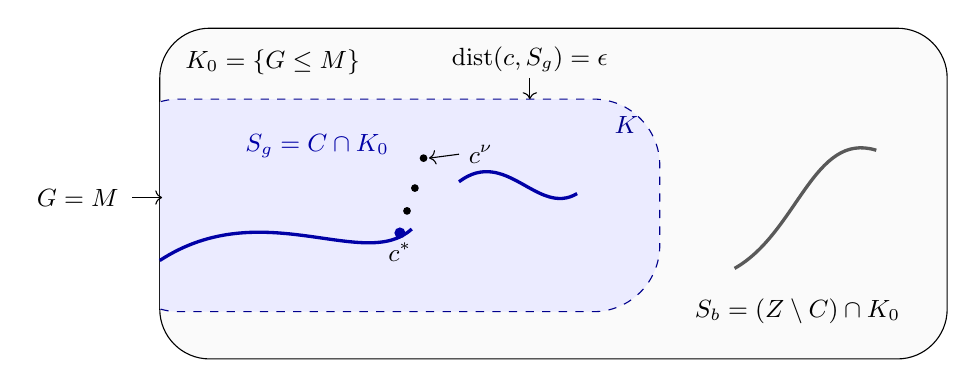
\begin{tikzpicture}[x=1cm,y=1cm, font=\small]
 \draw[rounded corners=18pt,fill=black!2] (0,0) rectangle (10,4.2);
 \node[anchor=north west] at (.2,4.05) {$K_0=\{G\le M\}$};
 \begin{scope}
 \clip[rounded corners=18pt] (0,0) rectangle (10,4.2);
 \draw[rounded corners=24pt,fill=blue!8,draw=blue!55!black,dashed]
   (-.6,.6) rectangle (6.35,3.3);
 \end{scope}
 \node[anchor=north east,text=blue!55!black] at (6.2,3.2) {$K$};
 \draw[very thick,blue!65!black] (0,1.25) .. controls (1.3,2.1)
   and (2.6,1.1) .. (3.2,1.65);
 \draw[very thick,blue!65!black] (3.8,2.25) .. controls (4.4,2.7)
   and (4.8,1.8) .. (5.3,2.1);
 \node[text=blue!65!black] at (2,2.7) {$S_g=C\cap K_0$};
 \node[anchor=east] at (-.4,2.05) {$G=M$};
 \draw[->] (-.35,2.05) -- (.03,2.05);
 \node at (4.7,3.8) {$\operatorname{dist}(c,S_g)=\epsilon$};
 \draw[->] (4.7,3.57) -- (4.7,3.3);
 \draw[very thick,black!65] (7.3,1.15) .. controls (8.1,1.6)
   and (8.3,2.9) .. (9.1,2.65);
 \node[align=center] at (8.1,.6) {$S_b=(Z\setminus C)\cap K_0$};
 \fill[blue!65!black] (3.05,1.6) circle (2pt);
 \node[below] at (3.05,1.6) {$c^*$};
 \fill (3.35,2.55) circle (1.4pt);
 \fill (3.24,2.17) circle (1.4pt);
 \fill (3.14,1.88) circle (1.4pt);
 \draw[->] (3.8,2.6) -- (3.42,2.55);
 \node[anchor=west] at (3.8,2.6) {$c^\nu$};
\end{tikzpicture}
\caption{The compact-neighborhood argument, schematically.  The selected
zero set $S_g$ and the excluded zero set $S_b$ are separated inside
$K_0$.  The set $K$ can meet the boundary $G=M$.  Penalized minimizers
converge to $c^*\in S_g$ with $G(c^*)<M$ and distance zero from $S_g$,
strictly below $\epsilon$.  They are therefore eventually interior to
$K$, away from both boundary portions.  The drawn shapes assert no
smoothness or connectedness of these sets.}
\label{fig:compact-neighborhood}
\end{figure}

Apply Proposition~\ref{prop:candidate-coordinates} to $W=W_d$ and to
the good part of $Z_d$.  We use $c=(x,t)\in\R^{r+1}$ and choose
$\ell$ from a uniform short degree bound on $W_d$.  Whenever this good
part is nonempty, it contains a point whose coordinates are roots of
the nonzero coefficient polynomials $P_{i,j_i}$.  These polynomials
are controlled uniformly in $d,i,j_i$.

\subsection{The final decision}

We can now use root labels to replace the real choice of $x$ by short
discrete data.  Choose an integer $0\le d\le d_E$ and, for each
$1\le i\le r+1$, an index $j_i$ within a uniform short bound on the
$w$-degree of $P_i$.  For each $P_{i,j_i}$ choose root-label data as
in Proposition~\ref{prop:root-labels}, with the auxiliary positivity
test equal to $1$, and write $L_i$ for the resulting controlled
polynomial.  Let $\mathcal S(c)$ denote the conjunction
\begin{equation}\label{eq:selected-coordinates}
 W_d(c)=0,\qquad
 P_{i,j_i}(c_i)=0,\qquad L_i(c_i)>0
 \quad(1\le i\le r+1).
\end{equation}
For these choices, accept exactly when both statements hold:
\begin{align}
 &\exists c\in\R^{r+1}\;\mathcal S(c),
 \label{eq:final-nonempty}\\
 &\neg\exists(c,z)\in\R^{r+1+n}\;
       \bigl(\mathcal S(c)\ \wedge\ F(x,z)=0\bigr).
 \label{eq:final-no-counterexample}
\end{align}
Each existential statement is an instance of
Theorem~\ref{thm:controlled-existential}.  Their conjunction, with
negation as displayed, is therefore an available decision.

We verify the two directions separately; they use the labels in
different ways.  If the test accepts, choose $c=(x,t)$ from
\eqref{eq:final-nonempty}.  Statement
\eqref{eq:final-no-counterexample} implies that $F(x,\cdot)$ has no
real zero.  Thus $x$ is good.  This implication holds for every choice
of the indices and labels, even if a selected coefficient polynomial
is zero or the conjunction selects more than one point.

Conversely, suppose a good $x$ exists.  Let $d$ be the actual degree
of $E(x,\cdot)$.  Then the good part of $Z_d$ is nonempty.
Proposition~\ref{prop:candidate-coordinates} supplies a point
$c^*=(x^*,t^*)$ in that part and highest nonzero coefficient indices
$j_i$ for which $P_{i,j_i}(c_i^*)=0$.  By
Proposition~\ref{prop:root-labels}, labels can be chosen to single out
each $c_i^*$ among the real roots of its coefficient polynomial.
For these choices, \eqref{eq:selected-coordinates} has exactly the
one solution $c^*$.  It satisfies
\eqref{eq:final-nonempty}, and goodness of $x^*$ gives
\eqref{eq:final-no-counterexample}.  Some discrete choices therefore
accept.  Notice that the decision procedure does not need to verify
that an index is highest or a coefficient polynomial nonzero: those
properties provide complete choices, whereas the two tests ensure
soundness for all choices.

Finally, all discrete choices together have polynomial encoding length.
There are only $r+1$ coefficient indices and labels; each degree bound,
index bound, and label bound is short.  The real variables and the
number of equations and positivity tests in
\eqref{eq:final-nonempty}--\eqref{eq:final-no-counterexample} are
polynomially bounded.  The controlled-polynomial rules are used in a
fixed order: construct $Q$ and $E$, extract their coefficients and form
$W_d$, construct the coordinate polynomials, form the labels, and apply
the two existential tests.  Each stage is uniform in its short indices;
none introduces a separate oracle or one counting level per index.
The existential quantification over the entire discrete choice tuple
thus preserves availability.  The resulting decision function belongs
to a fixed level of the counting hierarchy, independent of the input.
Malformed inputs were rejected in polynomial time, so this proves
Theorem~\ref{thm:main}.

\appendix
\section{An explicit level for the existential fragment}
\label{sec:existential-bound}

For an ordinary existential sentence, the polynomial to be tested is
explicitly listed after the quartic reduction.  This permits more precise
level accounting than the controlled-family formulation requires.
There is also a simpler root selection: we need to isolate some root below
a threshold, whereas the two-block argument needs to specify any prescribed
coordinate root.  The simpler selection yields the following refinement.

\begin{theorem}\label{thm:etr-bound}
For the circuit encoding of the existential theory of the reals used in
this paper,
\[
 \ETR\in\Clevel{26},
 \qquad \existsR\subseteq\Clevel{26}.
\]
\end{theorem}

We prove the bound using the preceding algebraic and counting tools,
with a short list of derivative conditions in place of the labels from
Section~\ref{sec:labels}.

\subsection{Selecting some root with few derivative conditions}

The distinction between selecting some root and selecting a prescribed
root is elementary but useful.  Derivative signs distinguish all real
roots by Lemma~\ref{lem:thom-separation}.  If only one root from a
nonempty set is needed, repeatedly keeping a smallest nonempty sign
class gives a much shorter description.

\begin{lemma}[Sparse root selection]\label{lem:sparse-selection}
Let $p\in\R[y]$ be a nonzero polynomial of degree $d\ge1$, and let
$S$ be a nonempty set of distinct real roots of $p$.  There is a list
of at most $\lceil\log_2|S|\rceil$ conditions
\[
 \sgn p^{(j)}(\alpha)=v,
 \qquad 1\le j\le d,\quad v\in\{-1,0,1\},
\]
satisfied by exactly one member of $S$.
\end{lemma}

\begin{proof}
If at least two roots remain, their derivative sign strings differ in
some coordinate.  That coordinate partitions the remaining roots into
at least two nonempty classes.  Record the condition defining a smallest
nonempty class and keep that class; its size is at most half the previous
size.  After at most $\lceil\log_2|S|\rceil$ repetitions exactly one
root remains.  If $|S|=1$, use the empty list.
\end{proof}

For an $\ETR$ instance $\exists y\,\Theta(y)$, apply
Lemma~\ref{lem:quartic-fibers} with no free parameters and with
$\Phi=\neg\Theta$.  Renaming the full variable tuple gives an explicitly
listed nonnegative polynomial $F\in\Z[x_1,\ldots,x_n]$ with
$n\ge1$ and degree at most four, whose real zeros encode truth of
the instance.
Use Proposition~\ref{prop:specialization} with $\ell=5$.
In its notation, $D=5^n$, $U=2^\sigma$, $R=2^\rho$, and
\[
 q(y)=\det(yI-M_{h_U})\in\Z[y]
\]
is monic and squarefree of degree $D$.  The original sentence is true
if and only if $q$ has a real root below $R$.
Take $K=\max(1,H+\sigma V)$ from that proposition, so
$\norm q\le2^K$ and $K$ is short and polynomial-time computable.
Although $U$, $R$, and the coefficients
of $q$ may have long binary expansions, their bound exponents are short.

Put $T=2+3n$.  A test list consists of $t$ pairs $(b_i,v_i)$, where
\[
 1\le t\le T,\qquad b_1(y)=R-y,\qquad v_1=1,
\]
and each subsequent $b_i$ is $q^{(j_i)}$ for some $1\le j_i\le D$,
with $v_i\in\{-1,0,1\}$.  A root matches the list when
$\sgn b_i(\alpha)=v_i$ for every $i$.  If a real root below $R$
exists, Lemma~\ref{lem:sparse-selection} applied to all such roots
gives a list matching exactly one real root.  Indeed, at most
$\lceil\log_2D\rceil\le3n$ derivative conditions suffice.
Every list has polynomial encoding length, since both $T$ and
$\log D$ are polynomially bounded.

\subsection{A polynomial detecting the list}

We next turn these conditions into a polynomial that is negative exactly
at matching real roots.  The construction is the rational sign
approximation of Lemma~\ref{lem:rational-sign}, now applied to only
polynomially many tests.

First we need a common range for their nonzero values.
Every complex root $\alpha$ of $q$ satisfies $|\alpha|\le2^{K+1}$,
and every test polynomial satisfies
\[
 \deg b_i\le D,
 \qquad \norm{b_i}\le2^{K+D^2+\rho+2}.
\]
For derivatives, the coefficient increase is bounded by
$D^D\le2^{D^2}$; the same displayed estimate covers $R-y$.
Set
\begin{equation}\label{eq:sparse-value-bounds}
 B_0=K+D^2+\rho+2+D(K+1),\qquad B=DB_0+2.
\end{equation}
Then $|b_i(\alpha)|\le2^{B_0}$.
For the lower bound, the eigenvalues of the integer matrix
$b_i(M_{h_U})$ are these values at the $D$ roots of $q$.
The product of its nonzero eigenvalues, up to sign, is a nonzero
coefficient of its monic integer characteristic polynomial, and so
has absolute value at least one.  Bounding the other factors by
$2^{B_0}$ gives
\begin{equation}\label{eq:sparse-value-range}
 b_i(\alpha)\ne0
 \quad\Longrightarrow\quad
 2^{-B}\le |b_i(\alpha)|\le2^B.
\end{equation}
This argument permits some test values to vanish.

Let $s=T+10$ and define
\begin{equation}\label{eq:sparse-approximant}
 P(z)=\prod_{j=-B}^{B}
 \left(2^{\max(0,j)}+2^{\max(0,-j)}z\right)^{2s},
 \qquad
 A(z)=\frac{P(z)-P(-z)}{P(z)+P(-z)}.
\end{equation}
By Lemma~\ref{lem:rational-sign}, the denominator is at least one
on the real line, $A(0)=0$, and Equation~\eqref{eq:sparse-value-range}
implies
\[
 |A(b_i(\alpha))-\sgn b_i(\alpha)|
 \le2\cdot3^{-2s}\le\frac1{8T}
 \qquad(q(\alpha)=0,\ \alpha\in\R).
\]
Consequently
\[
 \Psi(y)=4\sum_{i=1}^{t}(A(b_i(y))-v_i)^2-1
\]
is at most $-1+1/(16T)$ at a matching real root.  At any other
real root one difference in the sum has absolute value at least
$1-1/(8T)\ge7/8$, and therefore $\Psi\ge33/16$.

Clear the positive squared denominators by setting
\begin{align*}
 D_i(y)&=P(b_i(y))+P(-b_i(y)),\\
 N_i(y)&=P(b_i(y))-P(-b_i(y)),\\
 g_*(y)&=4\sum_{i=1}^{t}(N_i(y)-v_iD_i(y))^2
                 \prod_{j\ne i}D_j(y)^2
              -\prod_{j=1}^{t}D_j(y)^2.
\end{align*}
This is an integer polynomial, equal on the real line to
$\Psi\prod_iD_i^2$.  As every $D_i\ge1$, it satisfies
\begin{equation}\label{eq:sparse-sign-margin}
 \begin{cases}
  g_*(\alpha)\le-\tfrac12,&\text{if $\alpha$ matches the list},\\
  g_*(\alpha)\ge\tfrac12,&\text{otherwise},
 \end{cases}
 \qquad(q(\alpha)=0,\ \alpha\in\R).
\end{equation}
For one additional choice $e\in\{0,\ldots,D\}$ put
\begin{equation}\label{eq:sparse-product}
 g(y)=4Dg_*(y)+e,
 \qquad
 X=\det M_{g(h_U)}
   =\prod_{q(\alpha)=0}g(\alpha)\in\Z.
\end{equation}
The determinant identity is Lemma~\ref{lem:real-eigenline}.
The sign argument of Section~\ref{sec:existential}, applied to
$L=-g_*$, gives
\begin{equation}\label{eq:sparse-product-criterion}
 q\text{ has a real root below }R
 \quad\Longleftrightarrow\quad
 X<0\text{ for some test list and some }e.
\end{equation}
Indeed, every $e$ preserves the real-root signs.  A list matching
exactly one real root gives exactly one negative real factor;
some $e$ avoids every nonreal zero, since each of at most $D$
nonreal roots forbids at most one of the $D+1$ choices.
The conjugate pairs then contribute positive factors.
Conversely, a negative product has a negative real factor, whose
root matches the list and hence lies below $R$.

For the subsequent computations we record explicit short bounds.
Writing $m_*=2s(2B+1)$ for the degree of $P$, set
\begin{equation}\label{eq:sparse-size-bounds}
 \begin{split}
 d_g&=2Tm_*D,\\
 l_*&=m_*(2B+1),\\
 E_*&=2T(l_*+2)+16(D+T+2),\\
 m_X&=DE_*+1.
 \end{split}
\end{equation}
Then $\deg g\le d_g$ and $|X|\le2^{m_X}$.
For the first bound, every term in $g_*$ has $t$ squared factors,
each of degree at most $m_*D$.  For the second, at every complex root
$\alpha$ each base in $P(\pm b_i(\alpha))$ has modulus at most
$2^{2B+1}$.  Hence
\[
 |P(\pm b_i(\alpha))|\le2^{l_*},\qquad
 |D_i(\alpha)|,|N_i(\alpha)|\le2^{l_*+1},\qquad
 |N_i(\alpha)-v_iD_i(\alpha)|\le2^{l_*+2}.
\]
Therefore
\[
 |g(\alpha)|\le D(16T+5)\,2^{2T(l_*+2)}\le2^{E_*},
\]
which gives the asserted product bound.  All displayed bound
parameters use a fixed number of sums and products of short integers,
so are themselves short and polynomial-time computable.

\subsection{Accounting for the oracle levels}

The two multiplication-determinant computations now have an explicit
cost.  Set
\[
 \Omega=6(1+d_g),\qquad L_0=D\Omega+4n,\qquad
 \lambda=5L_0+4n+D^2+10.
\]
For every prime $p>\lambda$, Proposition~\ref{prop:char-coeff}
applies both to $h_U$, of degree at most six, and to $g(h_U)$,
of degree at most $6d_g$.  The larger cutoff is used for both
applications.  To recover $\sgn X$ we need only
$p\le Y=2\max(16,m_X,\lambda)^4$, as in
Proposition~\ref{prop:crt-sign}.  In particular every queried prime
has polynomial bit length.

For the first application, the relations $f_i(\cdot,U)$ and
the objective $h_U$ have direct polynomial-bit-time evaluations
modulo $p$.  Indeed, $\ell=5$ gives $a_i=20^i$, with polynomial
bit length.  The quartic $F$ and its first and second derivatives
have polynomial-size monomial lists.  The constants
$U\bmod p$ and $R\bmod p$ are computed by powering with the short
exponents $\sigma$ and $\rho$.  The Jacobian is an $n\times n$
determinant of directly evaluable entries.  Thus
Proposition~\ref{prop:char-coeff}, with $a=0$, computes the indexed
coefficients $q_k\bmod p$ of $q(y)=\sum_{k=0}^{D}q_ky^k$ in
$\Flevel8$.

For $1\le j\le D$,
\[
 q^{(j)}(y)=\sum_{k=j}^{D}q_k
       \left(\prod_{r=0}^{j-1}(k-r)\right)y^{k-j}.
\]
The falling factorial is in $\Flevel4$ by Lemma~\ref{lem:product};
the outer sum therefore gives derivative evaluations in
$\Flevel9$ by Lemma~\ref{lem:counting}.  This includes every
test $b_i$, since $R-y$ is directly evaluable.
Each factor of $P(b_i(y))$ in
Equation~\eqref{eq:sparse-approximant} is consequently in
$\Flevel9$.  The product lemma puts $P(\pm b_i(y))$ in
$\Flevel{13}$.  Since the list contains only polynomially many
tests, the formulas for $D_i,N_i,g_*$, and $g$ need only
polynomially many such calls and short arithmetic operations.
Thus $g(y)$, and then $g(h_U(x))$, are evaluable in
$\Flevel{13}$.  These expressions use only integer additions and
multiplications; their field evaluations never invert a test denominator.

The second application of Proposition~\ref{prop:char-coeff}, with
$a=13$ and $v=g(h_U)$, computes
\[
 X\bmod p=(-1)^D[y^0]\det(yI-M_{g(h_U)})\bmod p
\]
in $\Flevel{21}$.  The first application uses only the original
quartic and its critical equations; the second calls the first
through the evaluations of $g$.  This is a fixed sequence of two
applications, independent of $n$ and $D$.

By Proposition~\ref{prop:crt-sign} and
Equation~\eqref{eq:sparse-size-bounds}, the sign of $X$ is in
$\Flevel{24}$.  Lemma~\ref{lem:counting} then puts existence of
a test list and an $e$ with $X<0$ in $\Flevel{25}$.
Equation~\eqref{eq:sparse-product-criterion} therefore gives a
decision function for $\ETR$ at that level, and a language in
$\Clevel{26}$.  Polynomial-time many-one precomputation preserves
this level, proving the second assertion of Theorem~\ref{thm:etr-bound}.

\begin{table}[tb]
\centering
\begin{tabular}{lc}
\toprule
Quantity or decision & Sufficient class\\
\midrule
Indexed coefficients of $q\bmod p$ & $\Flevel8$\\
Derivative-test evaluations & $\Flevel9$\\
Evaluations of $P$, $g$, and $g(h_U)$ & $\Flevel{13}$\\
$X\bmod p$ & $\Flevel{21}$\\
$\sgn X$ & $\Flevel{24}$\\
Existence of a list and $e$ with $X<0$ & $\Flevel{25}$\\
Membership in $\ETR$ & $\Clevel{26}$\\
\bottomrule
\end{tabular}
\caption{A conservative level bound for the existential fragment.
Every indexed family uses a single uniform evaluator.}
\label{tab:existential-levels}
\end{table}

The shortness of all indices is independent of these level counts.
The bounds $D,K,\rho,\sigma,B,d_g,m_X,\lambda,Y$ are computed
in polynomial bit time, test lists have at most $T$ entries, and
every field element and product index has a polynomial-length
encoding.  Thus no long integer is passed as an explicit oracle
query, and Table~\ref{tab:existential-levels} describes fixed uniform
machines.

\bibliographystyle{plainnat}
\begingroup\raggedright\interlinepenalty=10000
\bibliography{references/references}
\endgroup
\end{document}
